%%%%%%%%%%%%%%%%%% USAGE INSTRUCTIONS %%%%%%%%%%%%%%%%%%
% - Compile using LuaLaTeX and biber, unless there is a particular reason not to. Do not use the older LaTex/PDFLaTeX or BibTeX. (The fonts won't work correctly.)
% - Expect to get 2 warnings when working correctly, one on xcolor and hyperref, and one on ExtSizes saying is better to use a class. These can be ignored.
% - Font and the report 'year' must be specified when all \documentclass or the template won't work correctly. (There's no error checking/default cases!)
% - For best performance save images/graphics as PDF files, not as png/jpg/eps. This makes no difference to how images are inserted using \includegraphics.
% - As many further packages as wanted can be loaded. Below are just an example set. Note that template itself loads a number of packages, including hyperref.
% - References are handed using biblatex.
% - Link to the presentation of dissertations policy: https://documents.manchester.ac.uk/display.aspx?DocID=2863



%%%%%%%%%%%%%%%%%% META DATA SETUP %%%%%%%%%%%%%%%%%%
% This is where the document title and author are set. Other details for the title page are set later
% Note that if/when you edit these you may need to 'Recompile from scratch' to get the changes to display in the PDF. (In Overleaf, select the down arrow to the right of the 'Recompile' button)
\begin{filecontents*}{\jobname.xmpdata}
  \Title{An Area and Power-Efficient Bit-Serial SIMD Array Processor for Image Processing on FPGA} 
  \Author{11319192} % should be student number rather than name to help with annoymous marking
  \Language{en-GB}
  \Copyrighted{True}
  % More meta-data fielda can be added here if wanted, see https://ctan.org/pkg/pdfx?lang=en for fields
\end{filecontents*}


%%%%%%%%%%%%%%%%%% DOCUMENT SETUP %%%%%%%%%%%%%%%%%%
\documentclass[12pt,beng]{uom_eee_dissertation_casson} % course can be msc or beng
% Check your course handbook for the correct font size to use. Make sure this is correct - you may get an overlength penalty if not! Is currently 12 for BEng, and 11 for MSc. The template doesn't change this automatically for you


%%%%%%%%%%%%%%%%%% FONT SETUP %%%%%%%%%%%%%%%%%%
    \setmainfont[
        Path = ./,
        Extension = .ttf,
        UprightFont = calibri,
        BoldFont = calibrib,
        ItalicFont = calibrii,
        BoldItalicFont = calibriz,
        Ligatures = TeX
    ]{calibri}
    
%%%%%%%%%%%%%%%%%% PACKAGES AND COMMANDS %%%%%%%%%%%%%%%%%%

% Packages
\usepackage{graphicx}              % for adding graphics files
  \graphicspath{ {./images/} }
\usepackage{amsmath}               % assumes amsmath package installed
  \allowdisplaybreaks[1]           % allow eqnarrays to break across pages
\usepackage{amssymb}               % assumes amsmath package installed 
\usepackage{url}                   % format hyperlinks correctly
\usepackage{rotating}              % allow portrait figures and tables
\usepackage{multirow}              % allows merging of rows in tables
\usepackage{lscape}                % allows pages to be typeset in landscape mode
\usepackage{tabularx}              % allows fixed width tables
\usepackage{verbatim}              % enhanced version of built-in verbatim environment
\usepackage{footnote}              % allows more control over footnote environments
\usepackage{float}                 % allows H option on floats to force here placement
\usepackage{booktabs}              % improve table line spacing
\usepackage{lipsum}                % for adding dummy text here
\usepackage[base]{babel}           % required for lisum package
\usepackage{subcaption}            % for multiple sub-figures in a single float
\usepackage{siunitx}               % add SI units
% Add your packages here


% Custom commands
\newcommand{\degree}{\ensuremath{^\circ}}
\newcommand{\sus}[1]{$^{\mbox{\scriptsize #1}}$} % superscript in text (e.g. 1st)
\newcommand{\sub}[1]{$_{\mbox{\scriptsize #1}}$} % subscript in text
\newcommand{\otoprule}{\midrule[\heavyrulewidth]}
\newcolumntype{Z}{>{\centering\arraybackslash}X}  % tabularx centered columns 
% Add your custom commands here

\numberwithin{equation}{section} % Adds section numbering to equations  ``

%%%%%%%%%%%%%%%%%% REFERENCES SETUP %%%%%%%%%%%%%%%%%%

% Setup your references here. Change the reference style here if wanted
\usepackage[style=ieee,backend=biber,backref=true,hyperref=auto,maxbibnames=3,minbibnames=1]{biblatex}
% Note backref=true adds a page number (and hyperlink) to each reference so you can easily go back from the references to the main document. You may prefer backref=false if you need to stick strictly to a given reference style


% Fixes which can't be applied in the .cls file
\DefineBibliographyStrings{english}{backrefpage = {cited on p\adddot},  backrefpages = {cited on pp\adddot}}
%  \renewcommand*{\bibfont}{\large}


% Add more .bib files here if wanted
\addbibresource{references.bib}



%%%%%%%%%%%%%%%%%% AUTOMATIC WORD COUNT SETUP %%%%%%%%%%%%%%%%%%
% Automatically counts the words present and makes a \mywordcount variable. This is used later to automatically add the word count (which can be overridden if wanted)
% See https://www.overleaf.com/learn/how-to/Is_there_a_way_to_run_a_word_count_that_doesn%27t_include_LaTeX_commands%3F for info on what words are counted and how to control this. Any changes to what's counted need to be made in uom_thesis_casson.cls, in the \newcommand{\quickwordcount} command. The default doesn't count words in headings, captions, or references and so you may get slightly different numbers if use a different word count tool
% This can be a bit fragile. If it doesn't work, there's an option later on to just type in a numer
\quickwordcount{\currfilebase} % run word count. This just counts the words. Is displayed with the \wordcount command later



%%%%%%%%%%%%%%%%%% START DOCUMENT %%%%%%%%%%%%%%%%%%

% Don't edit these lines, title and author are automatically taken from the document meta-data defined above
\begin{document}
\makeatletter
\title{\xmp@Title}
\studentid{\xmp@Author}
\makeatother

% Set the below yourself
\course{Electronic Engineering}  % "Master of Science in" or "Bachelor of Engineering in "
                                                   % is added automatically
                                                   % Our BEng courses are: Electrical and Electronic Engineering, Electrical Engineering, and Mechatronic Engineering
                                                   % Our MSc courses are: Advanced Control and Systems Engineering, Advanced Control and Systems Engineering with Extended Research, Communications and Signal Processing, Communications and Signal Processing with Extended Research, Electrical Power Systems Engineering, Advanced Electrical Power Systems Engineering, Renewable Energy and Clean Technology, Renewable Energy and Clean Technology with Extended Research, Robotics, Robotics with Extended Research
\faculty{Science and Engineering}                  % "Faculty of" is added automatically
\school{School of Engineering} % "School of" not added automatically (as if in AMBS, School comes at the end rather than the start), so enter full name of School here
\submitdate{2026}                                  % regulations ask only for the year, not month
\wordcount{\mywordcount}		                   % use \wordcount{} to set the count. Can just type in a number (e.g. \wordcount{1000}	if don't want to use the automatic count.) This is automatically displayed after the table of contents. 
\maketitle



%%%%%%%%%%%%%%%%%% LISTS OF CONTENT %%%%%%%%%%%%%%%%%%
\uomtoc
% other lists are not required, but can include \uomlof and \uomlot if really want to


%%%%%%%%%%%%%%%%%% ABSTRACT %%%%%%%%%%%%%%%%%%
\begin{abstract} % put abstract here.

    Image processing in edge-intelligent systems, such as wearable devices and remote sensors, demands high throughput when operating within low power envelopes. Using conventional sequential processor architectures introduces disproportionate area and energy costs for workloads whose parallelism is fundamentally data-level and spatial. This dissertation presents the design and analysis of a custom bit-serial SIMD array processor targeted at the optimisation of these three constraints for low-level image processing workloads.
    
    The architecture exploits data-level parallelism through a two-dimensional grid of processing elements with NEWS connectivity, a 20-bit instruction set supporting movement-based convolution, and a distributed register file mapped to LUTRAM to minimise per-PE footprint. The design is implemented on a Xilinx XC7Z020 (PYNQ-Z2), characterised across five array configurations from 4 to 1024 PEs, and evaluated on Sobel edge detection and a shallow MNIST convolutional classifier. At 1024 PEs the processor delivers a word-level throughput of 2.42 GOPS at 71 MHz while consuming 92 mW and occupying 47.1\% of available LUTRAM and 31.7\% of logic LUTs. Peak energy efficiency reaches 0.0507 GOPS/mW at intermediate configurations. Three architectural bottlenecks, the single-word memory interface, OR-tree depth, and AXI-Lite handshake latency, are quantified with targeted architectural solutions proposed. The results demonstrate that fine-grained bit-serial SIMD remains a competitive operating point for area and power constrained image processing on FPGAs.

\end{abstract}%
\clearpage

%%%%%%%%%%%%%%%%%% List of Figures %%%%%%%%%%%%%%%%%%
\uomlof

%%%%%%%%%%%%%%%%%% List of Tables %%%%%%%%%%%%%%%%%%
\uomlot

%%%%%%%%%%%%%%%%%% List of Abbreviations %%%%%%%%%%%%%%%%%%
\clearpage
\phantomsection
\addcontentsline{toc}{section}{List of Abbreviations}
\section*{\bfseries\Large List of Abbreviations}
\begin{tabbing}
\hspace{3.5cm}\=\kill
\textbf{ALU}     \> Arithmetic Logic Unit \\
\textbf{ASIC}    \> Application-Specific Integrated Circuit \\
\textbf{AXI}     \> Advanced eXtensible Interface \\
\textbf{BRAM}    \> Block Random Access Memory \\
\textbf{CLB}     \> Configurable Logic Block \\
\textbf{CNN}     \> Convolutional Neural Network \\
\textbf{CPI}     \> Cycles Per Instruction \\
\textbf{FPGA}    \> Field-Programmable Gate Array \\
\textbf{FSM}     \> Finite State Machine \\
\textbf{GOPS}    \> Giga-Operations Per Second \\
\textbf{ISA}     \> Instruction Set Architecture \\
\textbf{LUT}     \> Look-Up Table \\
\textbf{LUTRAM}  \> Look-Up Table Random Access Memory \\
\textbf{MAC}     \> Multiply-Accumulate \\
\textbf{MIMD}    \> Multiple Instruction, Multiple Data \\
\textbf{MNIST}   \> Modified National Institute of Standards and Technology \\
\textbf{NEWS}    \> North, East, West, South \\
\textbf{PE}      \> Processing Element \\
\textbf{PISO}    \> Parallel-In Serial-Out \\
\textbf{ReLU}    \> Rectified Linear Unit \\
\textbf{RTL}     \> Register Transfer Level \\
\textbf{SIMD}    \> Single Instruction, Multiple Data \\
\textbf{SIPO}    \> Serial-In Parallel-Out \\
\end{tabbing}
\clearpage

%%%%%%%%%%%%%%%%%% DECLARATIONS %%%%%%%%%%%%%%%%%%
\begin{uomoriginality}
  \uomoriginalitydeclaration 
  % If the standard originality decalaration is sufficient, saying no portion of the work has been submitted in support of an application for another degree or qualification, the above command will automatically add the required text and nothing else is needed in this section.
  % If the standard statment isn't sufficient, then comment out the \uomoriginalitydeclaration command and type in your own text here explaining the authorship of any re-used portions. 
\end{uomoriginality}
\uomcopyrightstatement



%%%%%%%%%%%%%%%%%% ACKNOWLEDGEMENTS %%%%%%%%%%%%%%%%%%
\begin{uomacknowledgements}
I would like to thank my project supervisor Dr. Piotr Dudek for his amazing guidance and invaluable expertise, throughout this project.

\end{uomacknowledgements}



%%%%%%%%%%%%%%%%%% Start content %%%%%%%%%%%%%%%%%%
\uomstartmainbody % Don't delete. used to flag to the hyperlinks in the PDF that the main content is  starting



%%%%%%%%%%%%%%%%%% INTRODUCTION %%%%%%%%%%%%%%%%%%
\section{Introduction} % can use \input{} or \include{} for each section to draw content from other files rather than having everything in one big file

        Critical edge applications such as wearable medical devices, and remote sensors, must operate within constrained power and space limits while responding in real time. These devices cannot rely on processing on cloud servers because transmitting data can be slow or unreliable. Edge-intelligent systems address this by processing data locally, allowing for fast computation whilst minimising power and area consumption. To meet these requirements, parallel processor arrays (PPAs) and SIMD architectures are well suited. Their grid-like structure and ability to run many calculations in parallel make them ideal for tasks such as image processing in real-time embedded systems.

    \subsection{Background and Motivation}
        Image processing is the core workload of various edge systems. 2D convolution is the fundamental operation found in low-level vision and convolutional neural network (CNN) tasks. This is where a weighted sum of a pixel and its neighbours are repeated across the entire image. A single 3×3 convolution on a modest 256×256 image already requires over half a million multiply-accumulate (MAC) operations, and modern CNNs scale this by orders of magnitude through multiple stacked convolutional layers and feature channels. Executing such workloads on conventional sequential processors is very inefficient. Pipelining, superscalar issue, and out-of-order execution all target instruction-level parallelism, but they do not exploit the property that the same operation is applied independently to many data elements.

        Single-Instruction-Multiple-Data (SIMD) array processors exploit this property directly. A grid of processing elements (PEs) executes one shared instruction across many pixels in parallel, eliminating the per-instruction fetch and decode cost. When the array is connected through nearest-neighbour links, the spatial structure of convolution maps onto the hardware without the need for global memory access. 
        

        \subsection{Aims and Objectives}\label{sec:aims}
        The aim of this project is to design, implement, and evaluate an area and power efficient FPGA-based bit-serial SIMD array processor capable of executing image-processing workloads. Each objective is benchmarked against prior bit-serial FPGA designs (where possible) and against three criteria: area efficiency (resource consumption per processing element), energy efficiency (operations per unit power, GOPS/mW), and performance (Giga Operations Per Second, GOPS). The objectives for the design are as follows:
        
        \begin{enumerate}
        
        \item \textbf{Bit-serial processing element:}\label{item:obj1} Design a simple processing element comprising a bit-serial ALU supporting arithmetic and boolean logic alongside a bit-serial register file. Success is defined as a functionally correct Processing Element (PE) that passes testcases across all supported ALU operations and performs proper reads and writes to the register file, while achieving a per-PE slice and Look-Up-Table (LUT) footprint competitive with prior bit-serial FPGA designs.
        
        \item \textbf{Scalable NEWS-connected array:}\label{item:obj2} Replicate the PE into a two-dimensional grid with North, East, West, South (NEWS) connectivity, with a configurable boundary padding scheme and PE activity gating for inactive elements. Success is defined as fitting a large array configuration, sized against current bit-serial processors, within the available resources, delivering throughput in GOPS that scales with PE count while keeping dynamic power consumption (in mW) low enough to yield a competitive GOPS/mW figure.
        
        \item \textbf{Hardware control unit and instruction set architecture:}\label{item:obj3} Develop an FSM-based controller with a minimal instruction set sufficient to run complex workloads, sequence bit-serial PE execution, and provide a ready/valid handshake to the host. Success is defined as full ISA coverage through workload execution, with the controller correctly driving all datapath control signals.
        
        \item \textbf{ARM-host system integration:}\label{item:obj4} Connect the array processor to the ARM Cortex-A9 on the PYNQ-Z2 using AXI-Lite for instruction delivery and a true-dual-port BRAM for data exchange. Success is defined as a working host-accelerator system in which C programs running on the ARM core can issue instructions and read back results, with the integration logic fitting within the target device alongside the full array.
        
        \item \textbf{Application demonstration and evaluation:}\label{item:obj5} Implement two image processing workloads on the completed system: a 3x3 Sobel edge-detection filter and a shallow convolutional neural network for MNIST digit classification. Success is defined as both workloads producing the expected results: visible edges in the Sobel output and predicted digits matching the input labels.
        
        \end{enumerate}
    
  \subsection{Report Structure}
   Section \ref{sec:Literature Review} examines the different approaches taken by researchers who have built SIMD processors, based on a review of the literature. Section \ref{sec:methods} describes the methodology in detail, including the processor architecture, as well as the instruction set, control mechanisms, system architecture and image processing algorithms. Section \ref{sec:results} presents benchmarking results, bottleneck discussion and a threats-to-validity analysis. Section \ref{sec:ProjectManagement} goes through the different management techniques used, such as Gantt charts, risk registers and CPD logs, to monitor progress and ensure the project remained on schedule. Finally, Section \ref{sec:conclusion} summarises the findings from all sections and discusses potential future improvements. 

%%%%%%%%%%%%%%%%%% LITERATURE REVIEW %%%%%%%%%%%%%%%%%%
\section{Literature review}\label{sec:Literature Review}

  \subsection{Introduction}
        Conventional sequential processors are designed to execute instructions one at a time. Improvements to the traditional processor have been made to accelerate data throughput and instruction execution. Techniques such as pipelining, superscalar and out of order execution have been utilised, however, these approaches primarily target instruction level parallelism and not data level parallelism. Array processors are built upon the SIMD paradigm described in Flynn's Taxonomy \cite{ref:Flynn1966}, where multiple PEs act upon different pieces of data based on a single shared instruction stream. This architecture is designed to perform high-throughput computations on large data arrays through exploiting data level parallelism for tasks like image processing. Common types of SIMD processors include array processors, pipelined processors, and associative processors. \cite{ref:Flynn1972}

        Array processors contain a regular structure of Processing Elements (PE). Each PE typically contains a local register or memory, an arithmetic logic unit (ALU), and commonly north, east, south, west cardinal communication channels to neighbouring PEs. This allows for efficient local data movement without relying on slower global memory accesses as large amounts of data can be computed within the PEs without the need for loading and storing to memory. These architectural features make array processors highly suitable for operations that involve spatial computations, where the resultant values depend on the current pixel as well as its neighbours. This dissertation will focus on architectures related to the SIMD array processor. 

    \subsection{A Review of SIMD Array Processors}
        Over the decades, SIMD array architectures have evolved from bit-serial designs to more complex word-parallel architectures capable of performing more sophisticated arithmetic operations and tasks. Differences in PE count, clock frequency, local memory size, and interconnect topology play a critical role in determining the performance and efficiency of each implementation. Examining these metrics shows that improvements have been made toward greater scalability, computational efficiency, and suitability for image processing workloads.
        
        \subsubsection{Performance Metrics and Architectural Features of Past Arrays}\label{sec:past-arrays}
        
        Several early array processors were designed around the bit-serial SIMD paradigm, where each PE operates on one bit per clock cycle, requiring multiple cycles to complete even a basic 8-bit arithmetic operation. This architectural trade-off was made intentionally. Through reducing the width of the buses within the PE, the effective area was reduced, allowing designers to integrate more PEs into a processor. The processors introduced in Table \ref{table:bitserial_processors} follow the bit-serial SIMD execution model.

        The latency of data movement between PEs is highly dependent on the interconnect topology. The Massively Parallel Processor (MPP) \cite{ref:MPP1998}, Geometric Arithmetic Parallel Processor (GAPP) \cite{ref:GAPP1990}, and Distributed Array Processor (DAP) \cite{ref:ICL_DAP1982} utilise a mesh connectivity topology, with each PE being connected to four of its neighbours. While being simple to implement, it was only efficient for local operations as shifting data across the array was computationally expensive. On the other hand, CM-1 \cite{ref:CM1_1989} and CM-2 \cite{ref:CM2_1987} used a hypercube routing method, organising PEs across an $n$-dimensional binary cube, thus reducing the hop count between distant nodes. In the 65,536-PE CM-2, a 16-dimensional hypercube meant the worst-case inter-PE distance was 16 hops, compared to 510 for the mesh topology.

        The GAPP ran at 0.0576 GOPS with 144 PEs on a single chip with 128 bits of local memory. It was intended for embedded image processing applications, hence the architecture focused on area and power consumption. The DAP increased the number of PEs and local memory size to 4,096, consequently, increasing the throughput to 0.759 GOPS compared to the GAPP.

        The MPP was a 128 x 128 mesh with 1K bits of local storage per PE. It reached 6.555 GOPS at 10 MHz on 8-bit data. The CM-1 followed in 1985, with 65,536 PEs connected by a hypercube topology, 5 MHz clock frequency but increasing the throughput to 8 GOPS. The CM-2 retained the same number of PEs with a slightly increased clock frequency compared to the CM-1 but drastically increased its throughput to 45.8 GOPS. due to the addition of floating-point chips (one per 32 PEs). This showed that dedicated arithmetic hardware offered more than simply increasing the number of PEs. 
        
            \begin{table}[H]
            \centering
            \caption[Bit-serial array processors]{Comparison of past bit-serial SIMD array processors for 8-bit processing.}
            \label{table:bitserial_processors}
            
            \begin{tabularx}{\linewidth}{ZZZZZZ}
            \toprule
            \textbf{Processor} & \textbf{Processing Elements} & \textbf{Clock (MHz)} & \textbf{PE Local Memory} & \textbf{Interconnect} & \textbf{Throughput (GOPS)}\\
            \midrule
            
            MPP & 16384 & 10 & 1K bits & 2D mesh & 6.554\\
            CM-1 & 65536 & 5 & 4K bits & Hypercube & 8\\
            CM-2 & 65,536 & 7 & 64K bits & Hypercube & 45.86 \\
            GAPP & 144 & 10 & 128 bits & 2D mesh & 0.0576\\
            DAP & 4096 & 5 & 4096 bits & 2D mesh & 0.759\\   
            
            \bottomrule
            \end{tabularx}
            \end{table}
    
        \subsubsection{Performance Metrics and Architectural Features of Modern Arrays}\label{sec:modern-arrays}
            Most modern parallel accelerators have shifted from the SIMD model of the historical arrays to MIMD or hybrid execution, driven by the workload diversity of machine learning training and inference \cite{ref:knowles2021,ref:sn40l2024}. The Graphcore GC200 \cite{ref:knowles2021,ref:graphcore_arch} integrates 1,472 independent multi-threaded tiles connected through a stateless all-to-all fabric, delivering 250~TFLOPS at FP16 with 900 MB of on-chip SRAM. The Cerebras WSE-2 \cite{ref:wse2,ref:lie2022cerebras} occupies the opposite extreme: 850,000 MIMD tiles in a 2D mesh on a single 46,225 mm$^2$ wafer, sustaining 7.5~PFLOPS. The SambaNova SN40L \cite{ref:sn40l2024,ref:sn40l_isscc} adopts a coarse-grained reconfigurable dataflow architecture, delivering 638 TFLOPS through a compiler-configured interconnect. SCAMP-5 \cite{ref:scamp5} is the principal exception to the MIMD trend: a 256x256 SIMD array of 65{,}536 mixed-signal PEs delivering over 500 GOPS at sub-watt power through tightly integrated sensing, memory, and compute. 
            
            Table \ref{table:modern_processors} summarises these designs. Of these, only SCAMP-5 is a direct architectural comparator to the present work; the others are included to characterise the broader landscape and the design pressures that motivated the shift away from SIMD.
            
        \begin{table}[H]
            \centering
            \caption[Modern array processors]{Comparison of modern array processors.}
            \label{table:modern_processors}
            
            \begin{tabularx}{\linewidth}{ZZZZZZ}
            \toprule
            \textbf{Processor} & \textbf{PEs} & \textbf{Clock (MHz)} & \textbf{PE Local Memory} & \textbf{Interconnect} & \textbf{Throughput}\\
            \midrule
            SCAMP-5~\cite{ref:scamp5}          & 65{,}536 & 10      & 20 registers & 2D mesh & 0.655~TOPS\\
            GC200~\cite{ref:knowles2021}       & 1{,}472  & 1{,}330 & 624~KiB                      & All to all & 250~TFLOPS \\
            WSE-2~\cite{ref:wse2}              & 850{,}000 & $\sim$850 & 48~KB                    & 2D mesh       & 7{,}500~TFLOPS \\
            SN40L~\cite{ref:sn40l_isscc}       & 1{,}040  & $\sim$1{,}000 & 520~MB Shared & Reconfigurable & 638~TFLOPS \\
            \bottomrule
            \end{tabularx}
        \end{table}

        \subsubsection{Bit-Serial SIMD on FPGA}
        \label{sec:bitserial-fpga}
            A small number of works have explored bit-serial SIMD specifically on FPGA, occupying a design point distinct from both the historical ASIC arrays of Section~\ref{sec:past-arrays} and the modern accelerators of Section~\ref{sec:modern-arrays}.
            Walsh and Dudek~\cite{ref:walsh2012} present a 32x32 bit-serial SIMD array on a Xilinx Virtex-5 (XC5VLX50), with each PE encapsulated in two CLBs (four slices) and connected through four-neighbour NEWS topology. The design operates at 150 MHz and achieves a peak bit-serial throughput of 153.6 GOPS, demonstrating binary and 8-bit greyscale image processing. The architecture targets compactness and raw frequency, and serves as the most direct comparator to the work presented in this dissertation.
            
            SPAR-2~\cite{ref:spar2} and its successor IMAGine~\cite{ref:imagine} take a different approach, pairing bit-serial ALUs with distributed BRAMs as a processing-in-memory overlay rather than a NEWS-connected mesh. SPAR-2 is a programmable overlay for machine learning workloads on edge FPGAs, while IMAGine reaches 737 MHz on AMD Alveo U55 hardware with 64K bit-serial MAC units, optimised for matrix-vector operations rather than pixel-parallel image processing.

        \subsubsection{Comparison Between Array Implementations}
            Three key trends emerge when comparing the architectures surveyed in Sections~\ref{sec:past-arrays}–\ref{sec:bitserial-fpga}. First, modern designs trade PE count for more complex PEs. The GC200 delivers over many orders of magnitude greater throughput than the MPP with fewer than one-tenth the PE count, although the comparison is across different precision regimes (FP16 versus 8-bit integer). Second, the choice of interconnect reflects the type of workload performed. 2D mesh architectures scale well in hardware, but they introduce communication delays between distant PEs. This is acceptable for locally connected tasks like CNNs (e.g., SCAMP-5 and WSE-2), where most data stays nearby. However, it becomes inefficient for operations that require all-to-all communication, like the GC200’s crossbar and the SN40L’s reconfigurable interconnect. Third, on-chip memory capacity has become the principal architectural differentiator. Off-chip DRAM accesses cost two to three orders of magnitude more energy per byte than SRAM~\cite{ref:horowitz2014} as well as possessing a longer data fetch latency. Bit-serial SIMD designs sidestep this trade-off by keeping data local to each PE, with movement handled through nearest-neighbour connectivity. The work presented in this dissertation is therefore not designed to compete with the modern accelerators of Section~\ref{sec:modern-arrays}. It positions itself most directly against the FPGA bit-serial designs of Section~\ref{sec:bitserial-fpga}, against which it is quantitatively compared in Section~\ref{sec:comparison}.
            
            \subsection{MNIST and Convolutional Neural Networks} 
            
            The Modified National Institute of Standards and Technology (MNIST) database is a collection of grey-scale images of handwritten digits. Constructed by LeCun \textit{et al.}\ from the larger NIST Special Databases~1 and~3, each digit is contained within a 20x20 box, and centred by mass within a 28x28 canvas~\cite{ref:lecun1998gradient}. The final dataset contains 60,000 training and 10,000 test examples, labelled with numbers ranging from 0 to 9~\cite{ref:deng2012mnist}. Its compact size and well-established baselines make it perfect for evaluating hardware accelerators. 
            
            \begin{figure}[H]
                \centering
                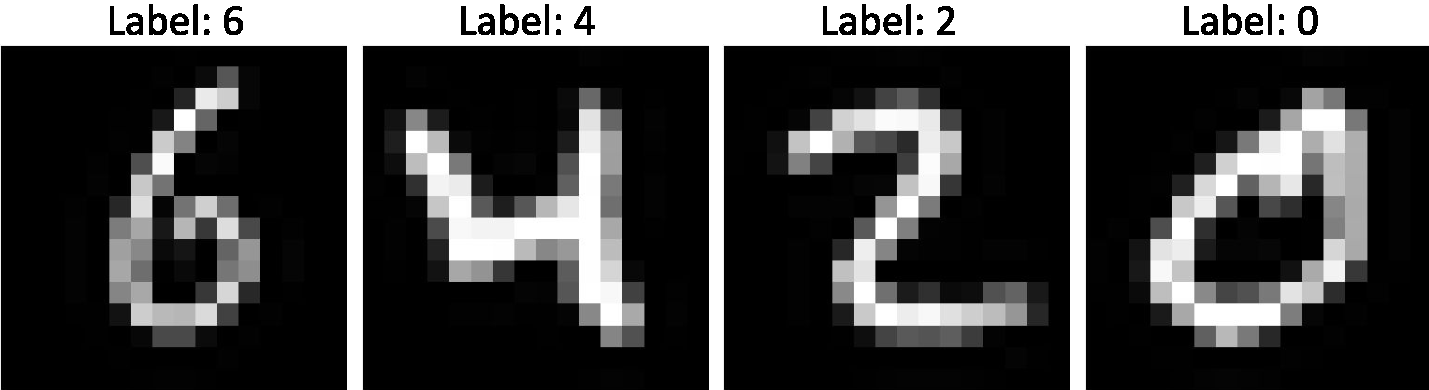
\includegraphics[width=\linewidth]{images/MNIST.pdf}
                \caption{Example labelled numbers from the MNIST dataset}
                \label{fig:placeholder}
            \end{figure}
            
            Convolutional Neural Networks (CNNs), trained end-to-end using back-propagation, make use of the spatial structure in image data through three key ideas: local receptive fields, shared weights, and spatial subsampling~\cite{ref:lecun1998gradient}. A classic example is \textit{LeNet-5}, introduced by LeCun \textit{et al.}\ in 1998, which combines convolutional and subsampling layers with fully connected layers for classification. It achieves less than $1\%$ error on the MNIST dataset~\cite{ref:lecun1998gradient}.
            
            The computation in CNNs is mainly made up of regular multiply--accumulate operations applied across 2D feature maps. This structure maps well onto a SIMD array, since the same operation is repeated independently across many pixels. In this design, the NEWS interconnect is used to pass data between neighbouring PEs, avoiding the need for global memory accesses during convolution. In addition, the bit-serial datapath allows precision to be adjusted depending on the layer, trading accuracy for performance when needed. Since MNIST inference is known to be robust to reduced precision, it is a suitable benchmark for evaluating the array processor, as discussed in Chapter~\ref{sec:results}.

    \subsection{PYNQ-Z2 Architecture}
    
    The PYNQ-Z2 is the chosen development board for this project, pairing a 650 MHz dual-core ARM Cortex-A9 with a Xilinx Zynq-7020 FPGA fabric containing 53,200 Look-Up Tables (LUTs), 106,400 flip-flops, and 140 Block RAMs \cite{ref:pynqz2}.
    
    The Zynq-7020 uses Xilinx's Advanced Silicon Modular Block (ASMBL) architecture, in which Configurable Logic Blocks (CLBs) are organised in columns alongside dedicated BRAM and DSP resources to improve routing efficiency \cite{ref:ug474}. Each CLB contains two slices, and slices come in two variants: SLICELs provide LUTs, flip-flops, multiplexers, and carry logic, while SLICEMs additionally allow their LUTs to be configured as shift registers or distributed RAM (LUTRAM) \cite{ref:ug474}.
    
    The SIMD array processor is synthesised entirely within the programmable logic, with each PE mapped onto LUT and flip-flop resources and inter-PE communication routed through the fabric. As the array scales, routing complexity and placement constraints become significant factors affecting achievable frequency and resource utilisation.


        \subsection{Summary}
        
        The literature review in this chapter demonstrates the evolution of parallel processing architectures from early bit-serial SIMD array processors to modern large-scale heterogeneous accelerators. While early designs prioritised simplicity and dense arrays of PEs, modern systems have shifted towards higher clock frequencies, deeper memory hierarchies, and more complex interconnects to achieve greater overall throughput.
        
        Despite these advances, data-level parallelism remains a fundamental principle across all architectures, particularly in workloads such as image processing and convolutional neural networks. However, existing approaches often trade architectural simplicity, power and area for performance, making them less suitable for edge applications where processors have to work under heavy constraints.
        
        Furthermore, while FPGA-based accelerators provide a flexible platform for implementing custom parallel architectures, they are constrained by limited on-chip resources, routing complexity, and a lack of domain-specific optimisation, all of which limit achievable PE density.
        
        This project addresses these gaps by implementing and evaluating a bit-serial SIMD array processor on an FPGA, focusing on its scalability, resource efficiency, and maintaining high performance for convolutional workloads such as MNIST inference.

%%%%%%%%%%%%%%%%%% METHODS %%%%%%%%%%%%%%%%%%
\section{Methods} \label{sec:methods}

  \subsection{Introduction}
    A simple overview of the entire system is shown in Figure \ref{fig:Brief_Full_System}.
    
\begin{figure}[H]
    \centering
    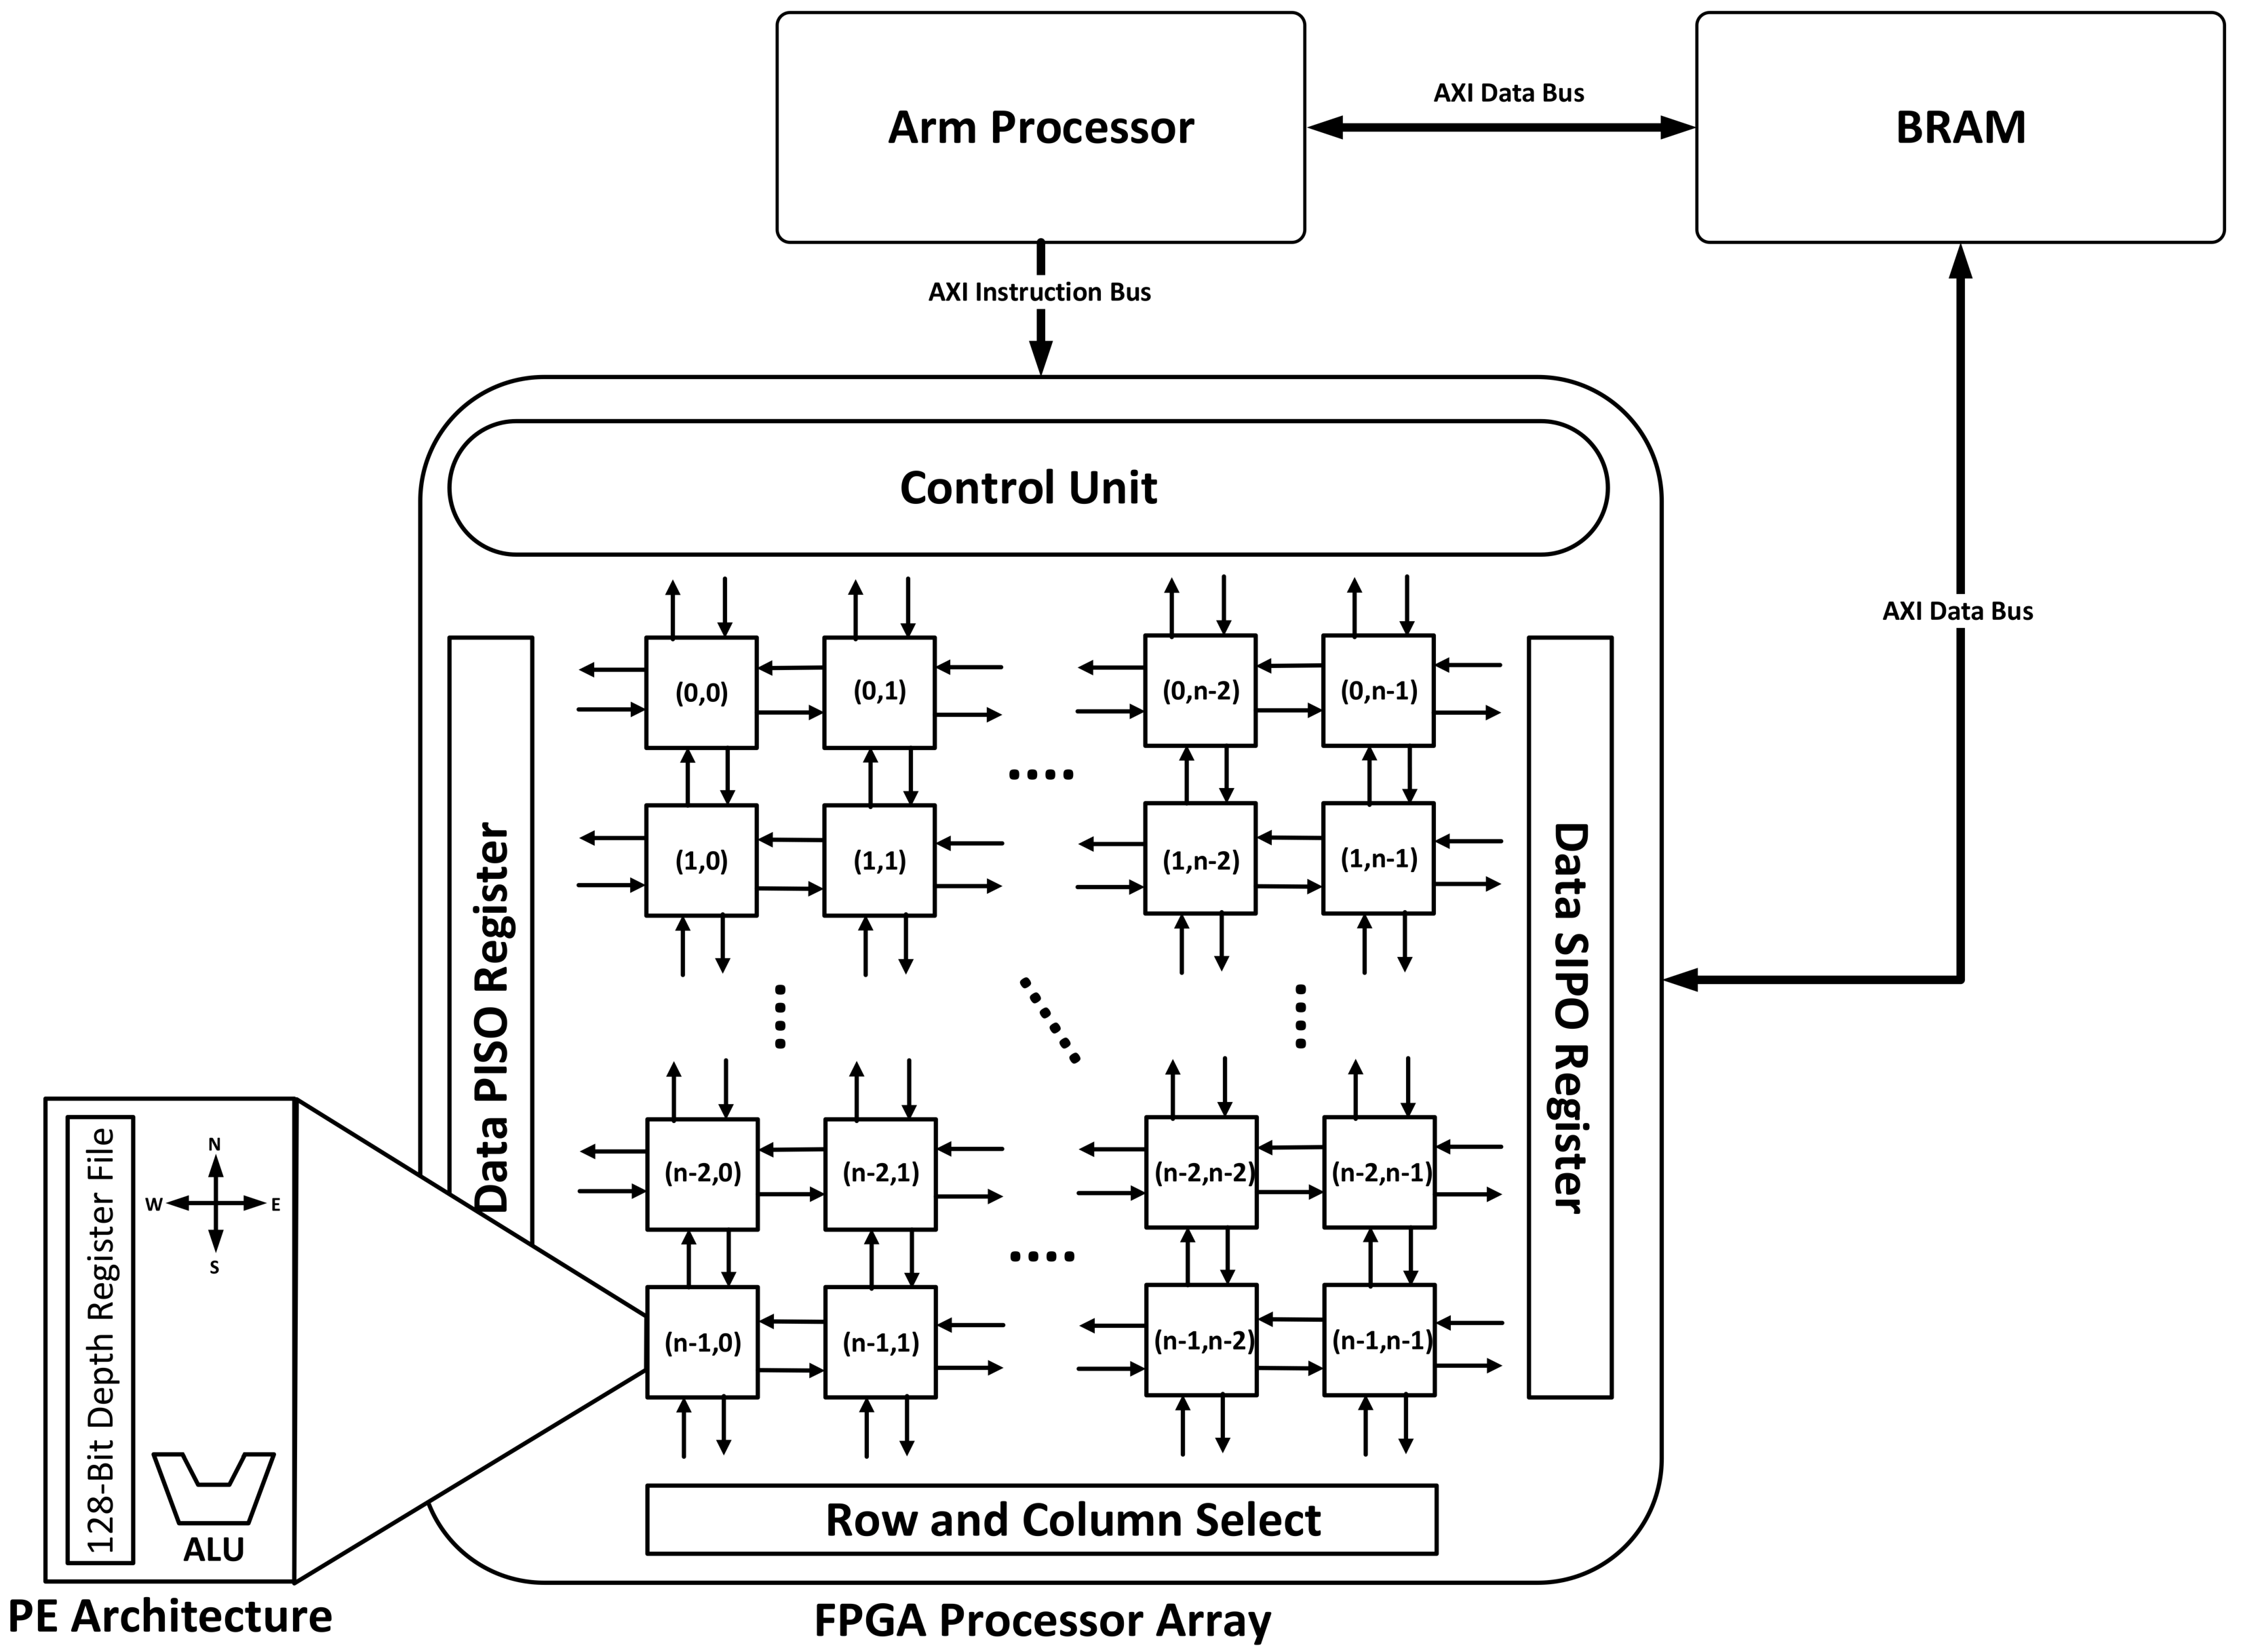
\includegraphics[width=0.7\linewidth]{images/Full_Individual_Project_Diagram.pdf}
    \caption{System and array processor overview}
    \label{fig:Brief_Full_System}
\end{figure}

    The processor consists of a grid of bit-serial PEs with NEWS connectivity driven by a hardware control unit. The control unit decodes 20-bit instructions and broadcasts control signals to all PEs. Each PE contains a bit-serial ALU, a register file, and a NEWS multiplexer for inter-PE communication, and is individually gated so inactive PEs do not contribute to dynamic power. An ARM processor issues instructions over an AXI instruction bus, while both the ARM and the array access shared BRAM via separate AXI data buses.

% \subsection{Content} \label{sec:content}
    \subsection{Array Architecture}
    
    The array (shown in Figure \ref{fig:Array_Architecture}) consists of a 2D grid of PEs and enabling scaling only in sizes that are powers of two. Each PE is connected to its four immediate neighbours and communicates via the North, East, West, and South (NEWS) channels. Boundary PEs can be supplied with zeros or ones. Input data, stored in 16-bit words in memory, is converted to a bit-serial format using a Parallel-In Serial-Out (PISO) register and fed into the array processor. A row and column select unit enables the selected PE to receive the data. The output data from the PEs are captured using an OR-reduction tree connected to a Serial-In Parallel-Out (SIPO) register. 
    
        \begin{figure}[H] %H means no floating image (must be placed after the text System Design
            \centering
            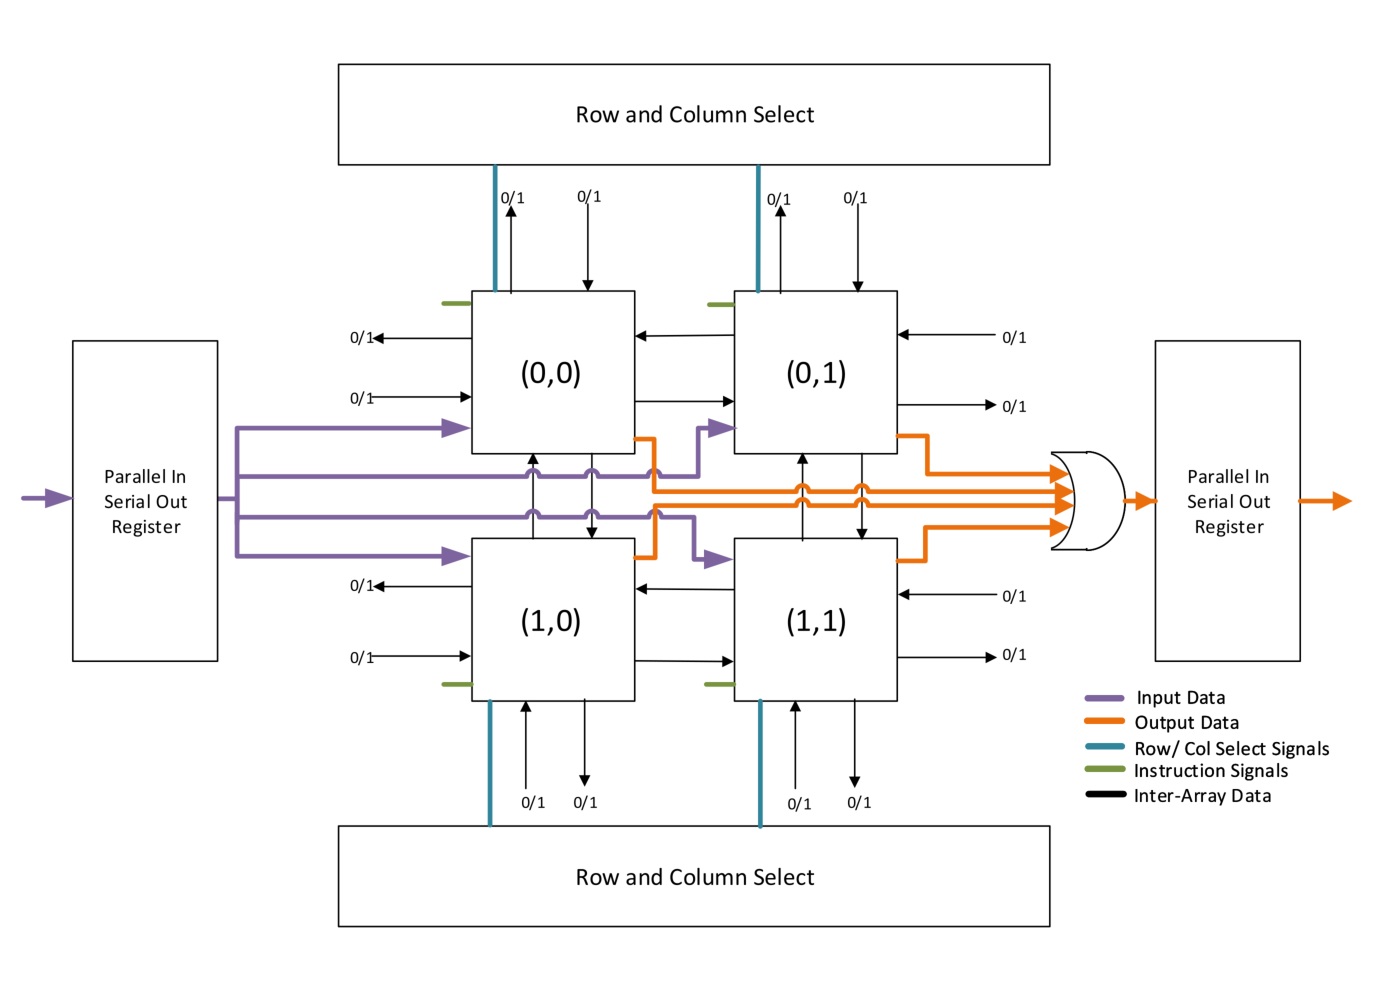
\includegraphics[width=\textwidth]{images/Array_Architecture.pdf}
            \caption{Array Processor High Level Architecture}
            \label{fig:Array_Architecture}
        \end{figure}
    
    The array implements pixel-parallel processing, assigning one pixel to each PE. For larger images, increasing the number of PEs to match the number of pixels can significantly improve data throughput. However, if the image size is smaller than the processor array, adding more PEs does not yield additional throughput. Conversely, if the number of PEs is smaller than the number of image pixels, processing time increases proportionally to the ratio of pixels to PEs. It is important to note that increasing the number of PEs also increases power consumption and overall resource utilization. 

    \subsection{Processing Element}
        All elements within each PE are implemented with bit-serial design principles. Each PE consists of an Arithmetic Logic Unit (ALU) and its own register file as shown in Figure \ref{fig:PE_Architecture}. 

        \begin{figure}[H] %H means no floating image (must be placed after the text System Design
            \centering
            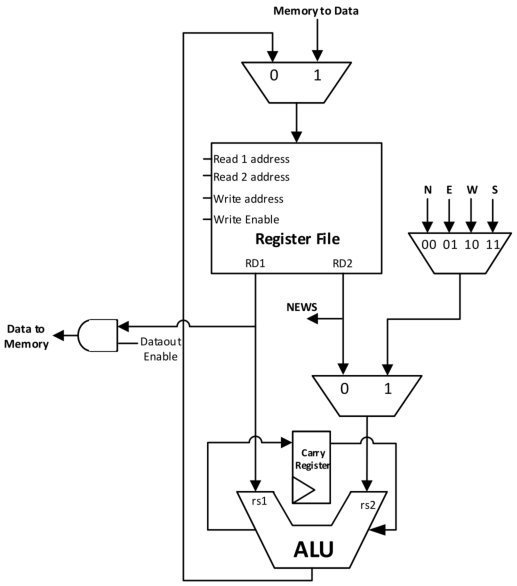
\includegraphics[width=0.6\textwidth]{images/PE_Architecture.pdf}
            \caption{Processing Element Datapath Architecture}
            \label{fig:PE_Architecture}
        \end{figure}

    
        \subsubsection{Arithmetic Logical Unit}
        The ALU performs addition starting from the least-significant bit (LSB). It implements the fundamental Boolean operations AND, OR and XOR. A full-adder structure is used for both addition and subtraction operations. Due to the bit-serial constraint of the architecture, the carry-out must be stored in a register and fed back as the carry-in for the next clock cycle, allowing carry propagation across word bits over multiple cycles. 
    
        \subsubsection{Register File}
        The register file is implemented in a bit-serial manner, organised as a one-dimensional structure with a depth of 128. This is done in a manner which allows the Vivado synthesis tool to infer LUTRAM with minimal resources. Individual bits are selected combinationally using a shared global counter as the bit index, which increments from 0 to 15 to extract a complete word LSB-first over 16 cycles.
        
        Two independent read ports are provided through combinational indexing. The first port supports arithmetic shift right function (SRA) by offsetting the bit index by a configurable shift amount to replicate the sign bit. The second port includes a bit-test mode (GETMSB) that bypasses the counter and stores 16 copies of the Most Significant Bit (MSB) into the destination register.
        
        Write operations share the same global counter as the bit index. When write enable is asserted, the incoming serial data bit is stored at the counter-indexed position within the destination register. Register zero is protected by gating the write enable. 
        
    \subsection{Control Unit}
        The control unit controls the data path and PE activities by generating the appropriate control signals for data path components such as the ALU, register file, memory subsystem, and inter-PE communication network, in accordance with the current instruction, while enforcing deterministic timing for each instruction class to ensure correct synchronisation and predictable execution across the architecture. The control unit is implemented in hardware and comprises a finite state machine (FSM) that sequences the instruction through its various execution stages, and a control decoder that generates the appropriate control signals based on both the current instruction and its execution state. 

        \subsubsection{Control Finite State Machine}   
        The Control FSM, as shown in Figure \ref{fig:FSM}, is responsible for sequencing instruction execution. Each state transition occurs on the rising edge of the clock and returns to an idle state upon an active-low reset.
        
        \begin{figure}[H] %H means no floating image (must be placed after the text System Design
            \centering
            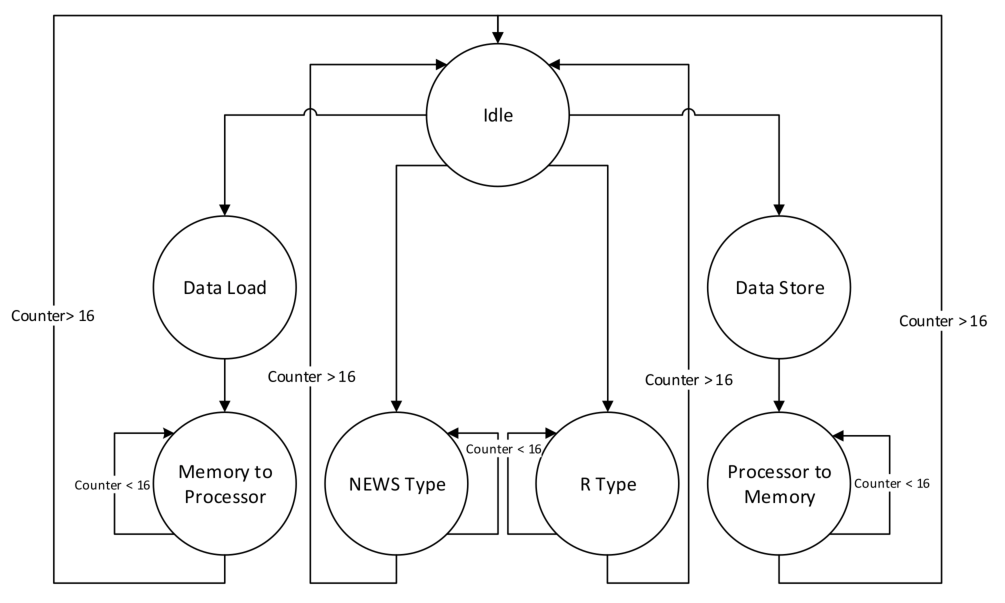
\includegraphics[width=0.8\textwidth]{images/FSM.pdf}
            \caption{Finite State Machine for the Array Processor}
            \label{fig:FSM}
        \end{figure}
        

        In the controller's idle state it inspects the opcode field, transitioning if it matches that of a specific instruction class and data valid signal is high. The data-valid signal, asserted by the ARM processor, indicates that a new instruction is ready. The supported instructions include load, store, arithmetic type (R-Type), and an inter-PE communication type (NEWS type).
        
        Multi-cycle instructions are managed using the global counter. During execution phases that require iterative processing, the counter increments on each clock cycle. Once 16 cycles have been completed, the instruction execution has completed and a new instruction is ready to be received
        
        For I/O operations (loads and stores), the control flow includes intermediate stages to manage data transfer between memory and the internal data-path. This is because an additional clock cycle is required for loading of PISO and SIPO registers before data enters/exits the array.
        
        A ready signal is asserted only when the FSM is in the idle state, providing a handshake mechanism for external logic. This ensures that new instructions are issued only when the controller has completed the previous operation.
        
        \subsubsection{Control Decoder}    
        The Control Decoder generates the control signals required to drive the data-path components. This is based on the current execution state provided by the Control FSM and the fields of the active instruction. While the FSM determines when a particular phase of execution occurs, the decoder determines how the data-path should behave during that phase. 

        During load operations, the decoder asserts the memory read control and generates the appropriate array memory address from the instruction’s immediate field. Data retrieved from memory is first parallel-loaded into a shift structure and then serially shifted into a select PE's destination register over multiple cycles. 
        
        For store operations, the decoder enables serial shifting of register data into the SIPO register before asserting a memory write control signal. The target memory address is constructed from the instruction’s encoded address fields, ensuring correct mapping within the array memory space. 
        
        For R-Type instructions, the decoder configures the ALU operation code using the instruction’s function fields. It selects the appropriate operand sources and enables all PEs and register write-back.
        
        In the case of inter-PE communication (NEWS-Type instructions), the operation is similar to the one specified by the R-Type instruction with the addition of a 2-bit combination sent to the NEWS mux to set the communication direction.
    
        \subsubsection{Instruction Set Architecture}
        The control architecture of the processor consists of four 20-bit instruction classes shown in Figure \ref{fig:Instr_Types}. Each instruction is uniquely identified by a 2 bit opcode located at the LSB positions of the instruction word. There are two primary I/O based instructions which facilitate memory-mapped addressing for individual PEs (loads and stores) and 2 for arithmetic and movement operations (R-Type and NEWS).
        
        \begin{figure}[H] %H means no floating image (must be placed after the text System Design
            \centering
            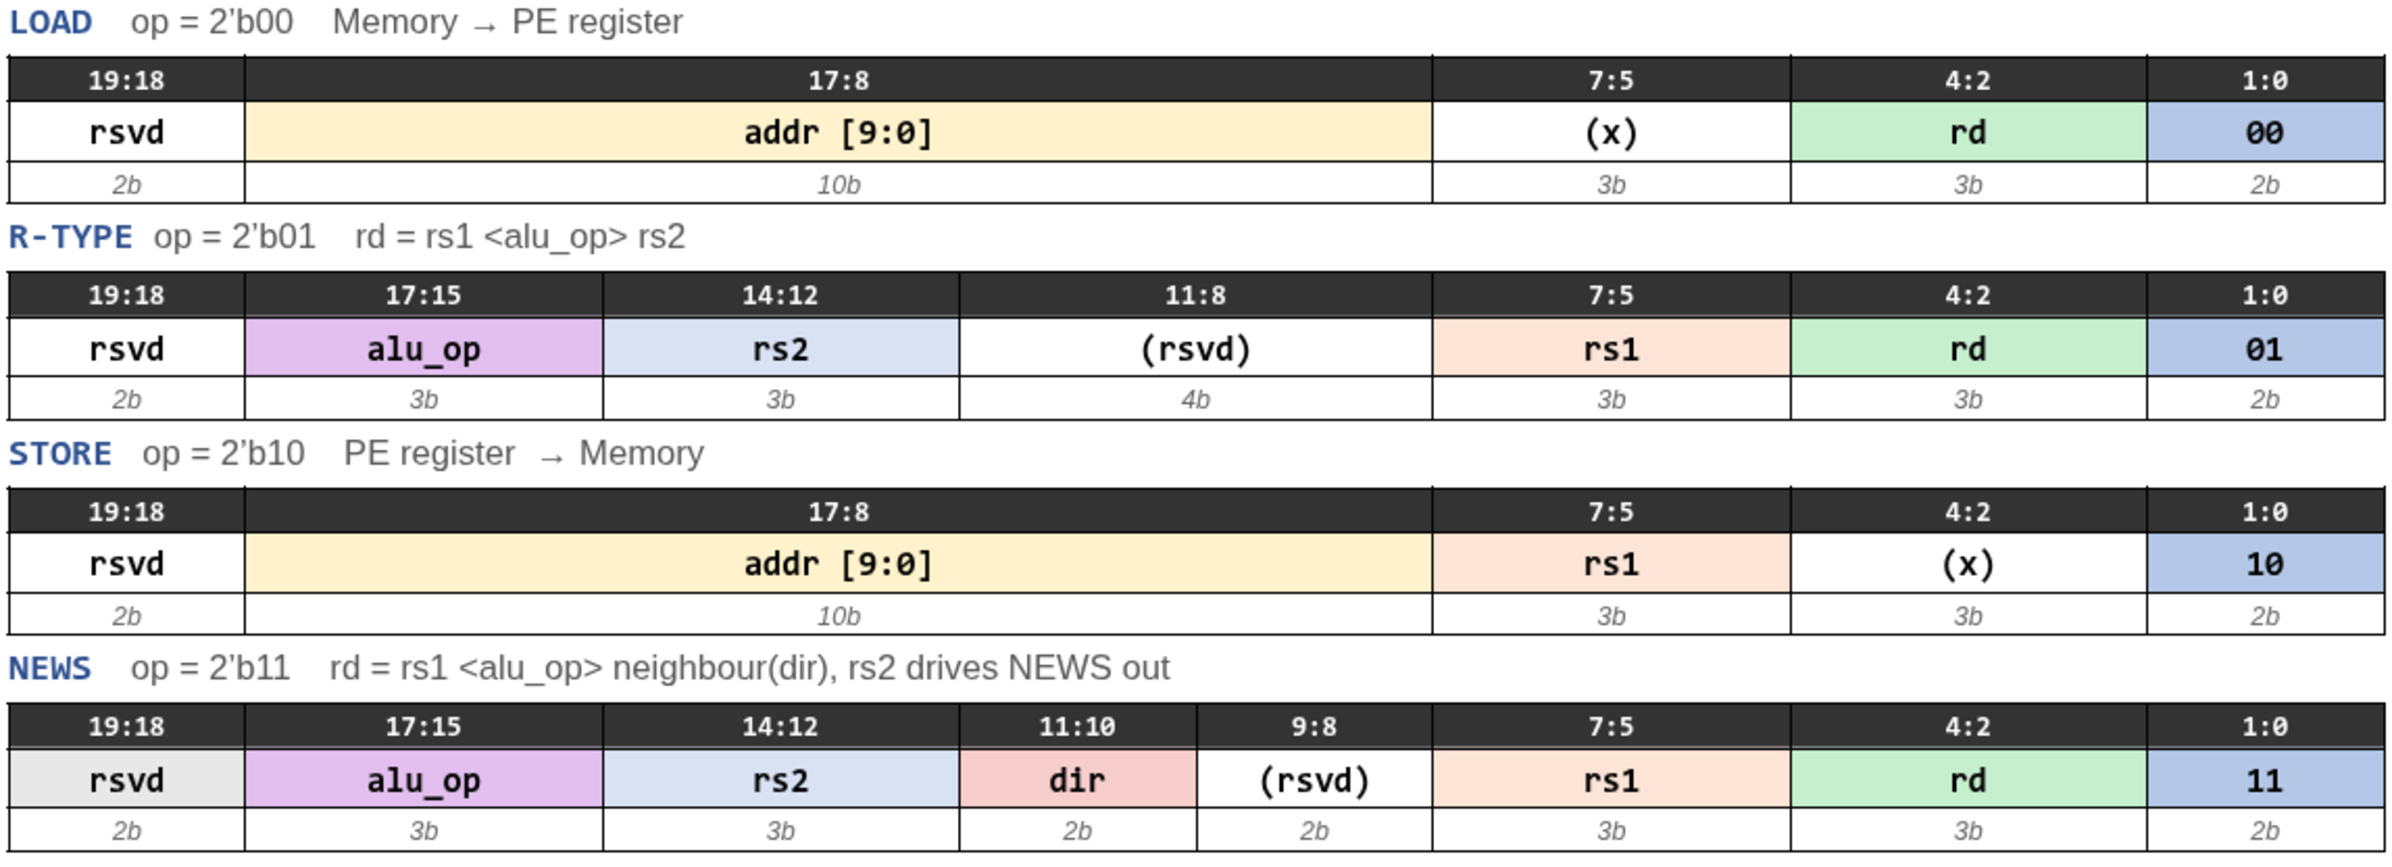
\includegraphics[width=\textwidth]{images/Instruction_Type.pdf}
            \caption{Instruction Types for the Array Processor}
            \label{fig:Instr_Types}
        \end{figure}

        Each I/O instruction encodes the memory address (addr) and either the source (rs1) or destination (rd) register of the PE. Both load and store operations complete in 18 clock cycles. The instruction types are designed so that the bit field encodings remain in the same bit position for different instructions, simplifying the decoding logic.
    
        In addition to memory operations, the architecture employs R-Type instructions to perform arithmetic and logical computations via the ALU using two register values as input operands. These operations are governed by a 3 bit identifier (alu\_op), allowing for the operations ADD, AND, OR, XOR, SUB, GETMSB and SRA to be implemented. All R-Type operations execute in 17 cycles corresponding to the word length. 
        
        The NEWS-Type instruction is used specifically for 2D array processing by leveraging 4-way connections between a PE and its neighbours. It contains a 3 bit ALU operation code (alu\_op) with two source operands (rs1 and rs2) and a destination register (rd). A direction specific field (dir) takes in 2 bits, allowing the 4 cardinal directions to be specified. Even with the data exchange and ALU operation, the instruction is completed in 17 cycles.  

        Table \ref{table:isa} summarises the instruction set architecture (ISA) and its corresponding C-level representations.
        \begin{table}[h]
        \centering
        \caption{Instruction Set Summary}
        \label{table:isa}
        \begin{tabularx}{\linewidth}{ZZZ}
        \hline
        \textbf{Instruction} & \textbf{Type} & \textbf{Description} \\
        \hline
        \texttt{vload(rd, imm)}                  & LOAD   & Load from memory into \texttt{rd} \\
        \texttt{vstore(rs1, imm)}                & STORE  & Store \texttt{rs1} to memory address \\
        \hline
        \texttt{vadd(rd, rs1, rs2)}              & R-Type & \texttt{rd = rs1 + rs2} \\
        \texttt{vsub(rd, rs1, rs2)}              & R-Type & \texttt{rd = rs1 - rs2} \\
        \texttt{vxor(rd, rs1, rs2)}              & R-Type & \texttt{rd = rs1 \^{} rs2} \\
        \texttt{vorr(rd, rs1, rs2)}              & R-Type & \texttt{rd = rs1 | rs2} \\
        \texttt{vandd(rd, rs1, rs2)}             & R-Type & \texttt{rd = rs1 \& rs2} \\
        \texttt{getmsb(rd, rs1)}                 & R-Type & \texttt{rd = msb(r1)}\\
        \texttt{vsra(rd, rs1, shamt)}            & R-Type & \texttt{rd = rs1 >> shamt} \\
        \hline
        \texttt{mv\{N|E|W|S\}add(rd, rs1, rs2)} & NEWS   & \texttt{rd = neighbour(dir) + rs2} \\
        \texttt{mv\{N|E|W|S\}sub(rd, rs1, rs2)} & NEWS   & \texttt{rd = neighbour(dir) - rs2} \\
        \hline
        \end{tabularx}
        \end{table}
        
    \subsection{System Design}
        Additional supporting components, as shown in Figure \ref{fig:System_Design}, are required alongside the array processor in order to simplify system programming and enable more complex operations to be performed. The PYNQ-Z2 development board integrates an ARM Cortex-A9 processor, which is used to communicate instructions to the array processor. Communication between the ARM processor, block RAM (BRAM), and the array processor is implemented using AXI-Lite interfaces, enabling memory-mapped communication. This approach simplifies system integration and allows additional peripherals to be integrated into the system architecture with minimal modification.
    
        \begin{figure}[H] 
            \centering
            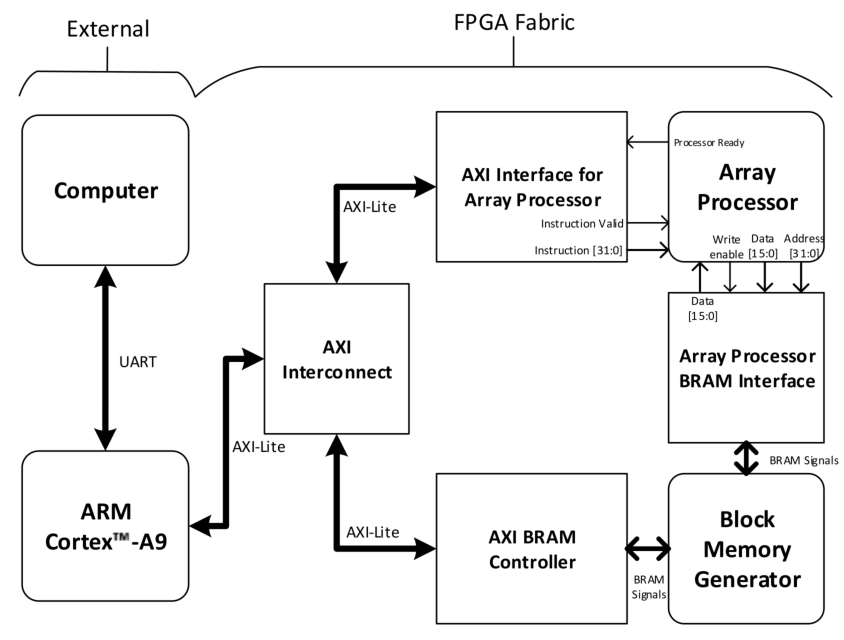
\includegraphics[width=0.75\textwidth]{System_Layout.pdf}
            \caption{System implementation for array processor. Important data, control and bus interface signals are presented. Bold arrows represent buses consisting of multiple signal types}
            \label{fig:System_Design}
        \end{figure}
  
        The ARM processor also provides the primary system clock for the design, while a processor system reset module generates the required reset signals for the different hardware components. Communication between the ARM processor and the host computer is performed via a UART interface, enabling the transmission of instructions and system control from the external machine.
        
        In addition to the processor subsystem, dedicated AXI and BRAM interfaces have been designed to enable communication between the processor and the on-chip memory. The AXI interface is used for the transmission of control signals between the processor and the array processor. For handshaking a processor-ready signal indicates that the current instruction has completed execution and, an instruction-valid signal is used to indicate the availability of a new instruction. An instruction is transmitted only when the ready signal is asserted and the instruction-valid signal experiences a rising edge, preventing repeating the same instruction execution.
        
        %include handshaking waveform
        
        The BRAM is configured as a true dual-port memory, allowing independent read and write operations to be performed simultaneously. The write enable (WEB) port is used to control write operations and to support different write widths when required. Read operations are performed when the enable signal is set to logic 0, while write operations occur when the signal is asserted to logic high. The BRAM interface accepts a 32-bit address, enabling access to a large memory space for instruction and data storage.

        %include hadshaking waveforms
  

    \subsection{Kernel Computation}\label{sec:Sobel}
        \subsubsection{Movement-Based Convolution on the Array}
        \label{sec:MB_Conv}
        A 2D convolution with a 3x3 kernel can be expressed as a 
        weighted sum of a pixel and its eight immediate neighbours. The full 
        derivation from the continuous convolution integral through to the 
        expanded discrete form is given in 
        Appendix~\ref{app:conv_derivation}. From this expansion, each kernel element $k_{i,j}$ at offset $(i, j)$ from the centre corresponds to a vertical shift $y \rightarrow y - i$, a horizontal shift $x \rightarrow x - j$, and a multiplication by the kernel weight (adopting the coordinate convention $y$-increases-downward, so a north shift is $y \rightarrow y - 1$). This structure maps onto the NEWS interconnect: horizontal shifts are realised as east/west movements between PEs, vertical shifts as north/south movements, and diagonals as compositions of the two (e.g.\ north-east is a north move followed by an east move).
        
        Applying this formulation to the Sobel operator removes the need for 
        a hardware multiplier entirely. The horizontal and vertical Sobel 
        kernels contain only the weights $\{-2, -1, 0, 1, 2\}$, and the 
        weighting factor of two can be produced by repeated summation of 
        shifted images rather than by multiplication. The detailed derivation 
        of the Sobel kernels in this movement-based form is given in 
        Appendix \ref{app:sobel_derivation}, and reduces the horizontal 
        gradient to the three-instruction sequence shown in 
        Listing \ref{code:Movement1}, with the vertical gradient following 
        the symmetric form in Listing \ref{code:Movement2}. 
        
        \begin{lstlisting}[language=Verilog, caption={Gx Kernel}, label={code:Movement1},
        basicstyle=\footnotesize\ttfamily,
        aboveskip=2pt,
        belowskip=2pt,
        xleftmargin=0pt,
        framexleftmargin=0pt]
        B = I + I(north)
        C = B + B(south)
        D = C(east) - C(west)\end{lstlisting}
        
        \begin{lstlisting}[language=Verilog, caption={Gy Kernel}, label={code:Movement2},
        basicstyle=\footnotesize\ttfamily,
        aboveskip=2pt,
        belowskip=2pt,
        xleftmargin=0pt,
        framexleftmargin=0pt]
        B = I + I(east)
        C = B + B(west)
        D = C(north) - C(south)\end{lstlisting}     
            
            \subsubsection{Algorithm for Sobel Edge Detection on 8-bit Greyscale Images}
            
            Using the derivation from Section \ref{sec:MB_Conv}, the horizontal Sobel gradient is obtained by first computing the vertically weighted column sum given in Equation \ref{eq:sobel_column_weight}.  
            The horizontal gradient is then formed by subtracting the west column from the east column as described in Equation \ref{eq:sobel_gx}.
            
            The vertical Sobel gradient is computed using the same weighting principle but with horizontal shifts, corresponding to the $G_y$ kernel in Equation \ref{eq:sobel_kernels}.
            
            The gradient magnitude is then approximated using the sum of absolute gradient values
            
            \begin{equation}
            O(x,y)=|G_x(x,y)|+|G_y(x,y)|
            \label{eq:sobel_output}
            \end{equation}

            This approximation avoids the computational cost of a square-root operation while still providing a reliable estimate of edge strength.
            
            Finally, the result is shifted right by three bits (division by 8) to ensure that the output value remains within the 8-bit range (0–255), since the maximum value produced by the preceding operations is 2040.
            
            As the algorithm relies only on neighbour shifts, additions, and subtractions, it maps efficiently to the proposed array processor architecture and enables parallel edge detection across the image.

    \subsection{MNIST Digit Classification}\label{sec:MNIST}
        The following sections describe the CNN model architecture and its implementation using the array processor's instruction set to classify MNIST digits.

        \subsubsection{CNN Model Architecture}  
        In this work, images from the MNIST dataset are rescaled from 28×28 to 16×16 pixels to align with the dimensions of the array processor. A 16×16 configuration is preferred over 32×32, as it enables efficient mapping without zero-padding, thereby avoiding unnecessary I/O overhead and underutilisation of processing elements that would arise when mapping a 28×28 input onto a larger array. Each greyscale pixel is then directly mapped to a corresponding processing element. The model was trained on the rescaled 16×16 dataset with weights quantised to Q1.7 fixed-point format, achieving 95.2\% accuracy on the MNIST test set.
        
        The classification model used in this work is a shallow Convolutional Neural Network (CNN). The network consists of a single convolutional layer with two output channels, followed by a max-pooling and a fully connected classification layer. The convolutional layer used two 3x3 kernels that are applied across the 16x16 input image. The boundary 2 rows/columns produced by zero-padded convolution are discarded, yielding a 14×14 valid region used by the classifier.
        
        Following the convolution stage, the Rectified Linear Unit (ReLU) activation function (as defined in equation \ref{eq:relu}) is applied after the convolution operation. This activation function was selected due to its implementation simplicity for the array processor.
        
        \begin{equation}
        f(x) = \max(0,x)
        \label{eq:relu}
        \end{equation}
        Here, $x$ denotes the input to the activation function, and $f(x)$ is the output after applying the ReLU non-linearity.
        
        Next, a 2x2 max-pooling operation is applied independently to each feature map shown in equation \ref{eq:maxpool}. This operation reduces the feature map size from 14x14 to 7x7, lowering the computational cost in subsequent processing stages.

        \begin{equation}
        y_{i,j} = \max \left(
        x_{2i,2j},\,
        x_{2i+1,2j},\,
        x_{2i,2j+1},\,
        x_{2i+1,2j+1}
        \right)
        \label{eq:maxpool}
        \end{equation}
        In equation \ref{eq:maxpool}, $x_{m,n}$ represents the input value at row $m$ and column $n$ of the feature map, while $y_{i,j}$ is the pooled output at row $i$ and column $j$.
        
        Following the pooling stage, the feature maps are flattened into a one-dimensional vector that forms the input to the fully connected layer.This layer computes a weighted sum of this vector according to equation \ref{eq:w_sum}, producing ten output activations corresponding to the ten digits 0 - 9. The predicted number is determined by selecting the output neuron with the highest value.

        \begin{equation}
          \hat{y} = \arg\max_{j \in \{0,\ldots,9\}} \left( b_j + \sum_{i=0}^{N-1} w_{i,j} \cdot x_i \right)
          \label{eq:w_sum}
        \end{equation}
        
        Here, $\hat{y}$ represents the index of the neuron with the maximum output activation, $x_i$ is the $i$-th input vector, $w_{ij}$ is the weight connecting input $i$ to neuron $j$, $b_j$ is the bias term of the $j$-th neuron, and $N$ is the total number of input features.
    
        The network architecture was intentionally designed to be lightweight in order to demonstrate the processor's capability to implement a CNN with high power and area efficiency. Using only two convolution channels significantly reduces the number of arithmetic operations and intermediate feature maps, while still achieving accurate digit classification. The CNN model was trained on a PC using the MNIST training dataset, and the resulting weights were extracted for inference.
        
    \subsection{Array Processor Implementation for MNIST Digit Classification}
        
        \subsubsection{System Memory Organisation}
        A dual-port block RAM (BRAM) serves as the shared memory interface between the host ARM Cortex-A9 and the array processor. The BRAM address space is partitioned into regions summarised in Appendix \ref{sec:memregalloc} Table \ref{tab:bram_map}.
        
        The host loads the 16 x 16 image into BRAM at initialisation, and the array processor reads or writes this memory through \texttt{vload}/\texttt{vstore} instructions, each
        addressed by a 10-bit PE identifier corresponding to a linearised row-major index.

        \subsubsection{Register Organisation}
        
        The image is loaded into \texttt{r1} by writing the pixel data to BRAM addresses 0--255 and issuing a corresponding stream of \texttt{vload} instructions. The register file allocation used throughout inference is shown in Appendix \ref{sec:memregalloc} Table \ref{tab:reg_alloc}.
        

        \subsubsection{Convolution Using Shift-and-Add Decomposition}
        As demonstrated by equation \ref{eq:conv_expanded}, each convolution requires the summation sequence of image shifts multiplied with a weight.

        Trained weights are interpreted as Q1.7 fixed-point fractions (i.e.\ $w/128$), so multiplication by a weight $w$ is realised by decomposing $|w|$ into a sum of powers of two and accumulating arithmetic right-shifts (\texttt{vsra}) of the operand. For a weight $w = 89$, for example, the decomposition $89 = 64 + 16 + 8 + 1$ yields four \texttt{vsra}/\texttt{vadd} pairs with shift amounts 1, 3, 4, and 7 respectively. Negative weights substitute \texttt{vsub} for \texttt{vadd}. This example is shown in Listing \ref{code:ConvMul} using the instruction encodings found in Table \ref{table:isa}
        
        A move to a cardinal neighbour is expressed as, for example,
        \texttt{mvsouthadd}$(dst, r_0, src)$, which shifts \texttt{src} one step northward (i.e.\ each PE receives the value from its southern neighbour) by exploiting the add-with-zero identity. Diagonal neighbours are reached by composing two orthogonal shifts. %put example here
        
        Following each complete convolution, a rescaling right-shift of three positions reduces the accumulator magnitude to ensure the values do not overflow before being passed to the activation function.

    \begin{lstlisting}[language=C, 
        caption={Example of multiplication by the (0,0) weight}, 
        label={code:ConvMul},basicstyle=\footnotesize\ttfamily,
        aboveskip=2pt,
        belowskip=2pt,
        xleftmargin=0pt,
        framexleftmargin=0pt]
    //position(0,0) weight=89
    issue(mvsouthadd(3, 0, 1));  // r3 = north(r1) + r0 = move
    issue(mveastadd(3, 0, 3));   // r3 = west(r3) = NW
    issue(vsra(4, 3, 7)); issue(vadd(2, 2, 4));
    issue(vsra(4, 3, 4)); issue(vadd(2, 2, 4));
    issue(vsra(4, 3, 3)); issue(vadd(2, 2, 4));
    issue(vsra(4, 3, 1)); issue(vadd(2, 2, 4));\end{lstlisting}

        \subsubsection{ReLU Activation}
        ReLU is implemented entirely with bitwise logic, avoiding any conditional branch or comparison instruction. The sign bit (MSB) of the accumulator is extracted and replicated across all 16 bits. A bitwise XOR with the all-ones mask then produces the inverse, yielding an all-zeros word when the accumulator is negative and an all-ones word when it is non-negative. An AND of this mask with the accumulator clamps negative values to zero while leaving positive values
        unchanged:
        
    \begin{lstlisting}[
        language=C,
        caption={ReLU activation},
        label={code:ReLU},
        basicstyle=\footnotesize\ttfamily,
        aboveskip=2pt,
        belowskip=2pt,
        xleftmargin=0pt,
        framexleftmargin=0pt
    ]
    getmsb(3, 2);       // r3 = sign(r2)
    vxor(3, 3, 7);      // r3 = ~sign(r2)
    vandd(2, 2, 3);     // r2 = r2 & r3 \end{lstlisting}


        
        \subsubsection{Max Pooling}
        A 2x2 stride-2 max-pooling operation is performed with two rounds. The source feature map is first copied into r1, each PE then computes the maximum of itself and its eastern neighbour, followed by the maximum of the updated value and its southern neighbour. Each pairwise maximum is computed without a comparator instruction by using the sign of the difference:

    \begin{lstlisting}[
        language=C,
        caption={Max Computation for Eastern Neighbour},
        label={code:maxpool},
        basicstyle=\footnotesize\ttfamily,
        aboveskip=2pt,
        belowskip=2pt,
        xleftmargin=0pt,
        framexleftmargin=0pt
    ]
    mvwestadd(2, 0, 1);    // r2 = east of r1
    vsub(3, 1, 2);         // r3 = self - east
    getmsb(4, 3);          // r4 = sign(self-east)
    vxor(5, 4, 7);         // r5 = ~sign
    vandd(3, 1, 5);        // r3 = self where self >= east
    vandd(5, 2, 4);        // r5 = east where east > self
    vorr(1, 3, 5);         // r1 = max(self, east) \end{lstlisting}
        
        After both rounds, r1 holds the 2x2 maximum at every PE. Stride-2 sampling is performed storing only the odd-indexed PE positions (rows and columns 1, 3, 5, 7, 9, 11, 13), extracting 49 pooled values per channel and writing them to their designated BRAM region. The two-channel pool therefore produces a 98-element feature vector.
        
        \subsubsection{Fully Connected Layer}
        The fully connected layer is executed on the host processor rather than the array processor, due to the lack of multiply-accumulate units. The host reads the 98 pooled values from BRAM and computes a dot product with each of the ten sets of FC weights, accumulating into a 32-bit integer score. A bias term is added for each class, and the class index achieving the maximum score is returned as the predicted digit as demonstrated by equation \ref{eq:w_sum}.
        
  \subsection{Summary}
    This chapter has presented the processor (for both the data-path and control), instruction set, system integration, and workload implementation for the array. The processor is built around a NEWS-connected grid of bit-serial PEs controlled by a unified hardware based control FSM and a 20-bit ISA, with LUTRAM-mapped register storage and AXI-Lite system integration. Two image-processing workloads, Sobel edge detection and a shallow MNIST CNN, demonstrate how the ISA can be used to run different workloads.
    
%%%%%%%%%%%%%%%%%% RESULTS %%%%%%%%%%%%%%%%%%
\section{Results and Discussion}    \label{sec:results}
    
    \subsection{Introduction}
    This chapter evaluates the bit-serial SIMD array implemented in Chapter~\ref{sec:methods} on a PYNQ-Z2 (Xilinx XC7Z020) platform. The analysis has three aims: to characterise the baseline performance of the design at a fixed configuration, to quantify how performance and resource cost scale with the three principal design parameters (array size, data-path width, and register-file depth), and to identify the bottlenecks that constrain efficiency.
    
    Two workloads are used to quantify the processor: a 3 x 3 Sobel edge-detection filter, executed on the 32 x 32 (1024-PE) configuration, and a shallow MNIST digit classifier, executed on the 16 x 16 (256-PE) configuration. The workloads are described in Sections~\ref{sec:Sobel} and~\ref{sec:MNIST} respectively. They were chosen as together they exercise every instruction class supported by the ISA and contain different data-movement patterns. The 16 x 16 configuration was used for the classifier rather than the maximum 32 x 32 because downscaling the MNIST input from 28 x 28 to 16 x 16 yields a 1:1 pixel-to-PE mapping without zero-padding overhead, while preserving sufficient spatial resolution for digit classification.
    
    Section~\ref{sec:Expmethodology} describes the measurement infrastructure and workload. Section~\ref{sec:baseline} presents the baseline characterisation in the default configuration (32 x 32 array, 16-bit datapath, register depth of 8). Section~\ref{sec:scaling} examines how area, power, and throughput are affected by scaling the number of PEs. Section~\ref{sec:imageResults} shows the results from running the two workloads and their execution times. Section~\ref{sec:comparison} compares against prior bit-serial SIMD designs, and Section~\ref{sec:discussion} discusses the results, bottlenecks, and identifies improvements.
    % ============================================================
    \subsection{Experimental Methodology}
    \label{sec:Expmethodology}
    
        \subsubsection{Simulation and Measurement Infrastructure} All functional and cycle-count results were obtained from a SystemVerilog simulation test-bench found in /Individual\_Project/sim within the Array Processor repository, as referenced in Appendix~\ref{sec:GitHub}. The repository README documents the purpose of each test-bench.
    
        To extract cycle counts per FSM state, an external module was introduced. It operates by tapping the current state signal and storing the number of clock cycle for each state. The per-instruction cycles-per-instruction (CPI) was obtained by counting cycles between successive rising edges of the control ready signal and categorising them based on the opcode field.
    
        Resource utilisation, achievable clock frequency (Fmax), and post-route power were obtained from Vivado utilisation report, timing summary, and power reports respectively. Power was estimated post-implementation using Vivado's vectorless analysis, which infers switching activity from default toggle-rate assumptions. Device static power is reported as the top-level leakage figure, which is an intrinsic property of the XC7Z020 at the estimated junction temperature.

    % ============================================================
    \subsection{Baseline Characterisation}
    \label{sec:baseline}
        All baseline results in this section are taken at the default configuration (32 x 32 array, data width of 16, and a register depth of 8. The number classification workload, characterised on the 16×16 configuration, is reported separately where indicated.

    \subsubsection{Per-PE Utilisation}
        Without Vivado's optimiser, each PE occupies 26 LUTs (18 logic LUTs and 8 LUTRAMs) when measured by applying the \texttt{keep\_hierarchy = "yes"} attribute to the PE module. This attribute prevents the synthesiser from merging logic across module boundaries. This represents the true per-PE cost before cross-boundary optimisation.
    
        When \texttt{keep\_hierarchy = "no"}, each PE utilises fewer LUT and slices. Due to Vivado's cross-boundary optimisation, per-PE LUT usage varies across the array with some PEs occupying 4 slices (2 SLICEM and 2 SLICEL) and some occupying 3 (2 SLICEM and 1 SLICEL). A test of a 16 x 16 grid of PEs revealed that, 227 (88.7\%) report 0 logic LUTs and 8 LUTRAMs, 28 (10.9\%) report 2 logic LUTs and 8 LUTRAMs, and one PE reports 1 logic LUT and 8 LUTRAMs, as the synthesiser merges combinational logic into neighbouring cells where possible. What remains constant across all PEs are 8 RAMD64E distributed-RAM cells implementing the register file, 4 MUXF7 wide-mux primitives building the register file's read path, and 1 flip-flop inferred for the carry register. In theory, up to 5184 PEs (72 × 72) could fit on the FPGA based purely on LUT availability. However, the PE array size must be a power of two, so the largest theoretically achievable configuration is 64 × 64. In practice, as shown in Section \ref{sec:scaling}, LUTRAM is the binding resource that limits scaling, reducing the maximum usable array to 32 x 32 PEs and occupying 47\% of the available LUTRAM.
        Figure \ref{fig:SLICES} shows the slices and the primitives inside of them used to build each PE. The two SLICEMs and the top-right SLICEL are consistent throughout all PEs while the top left SLICEL varies between PEs.
        
        \begin{figure}[H]
            \centering
            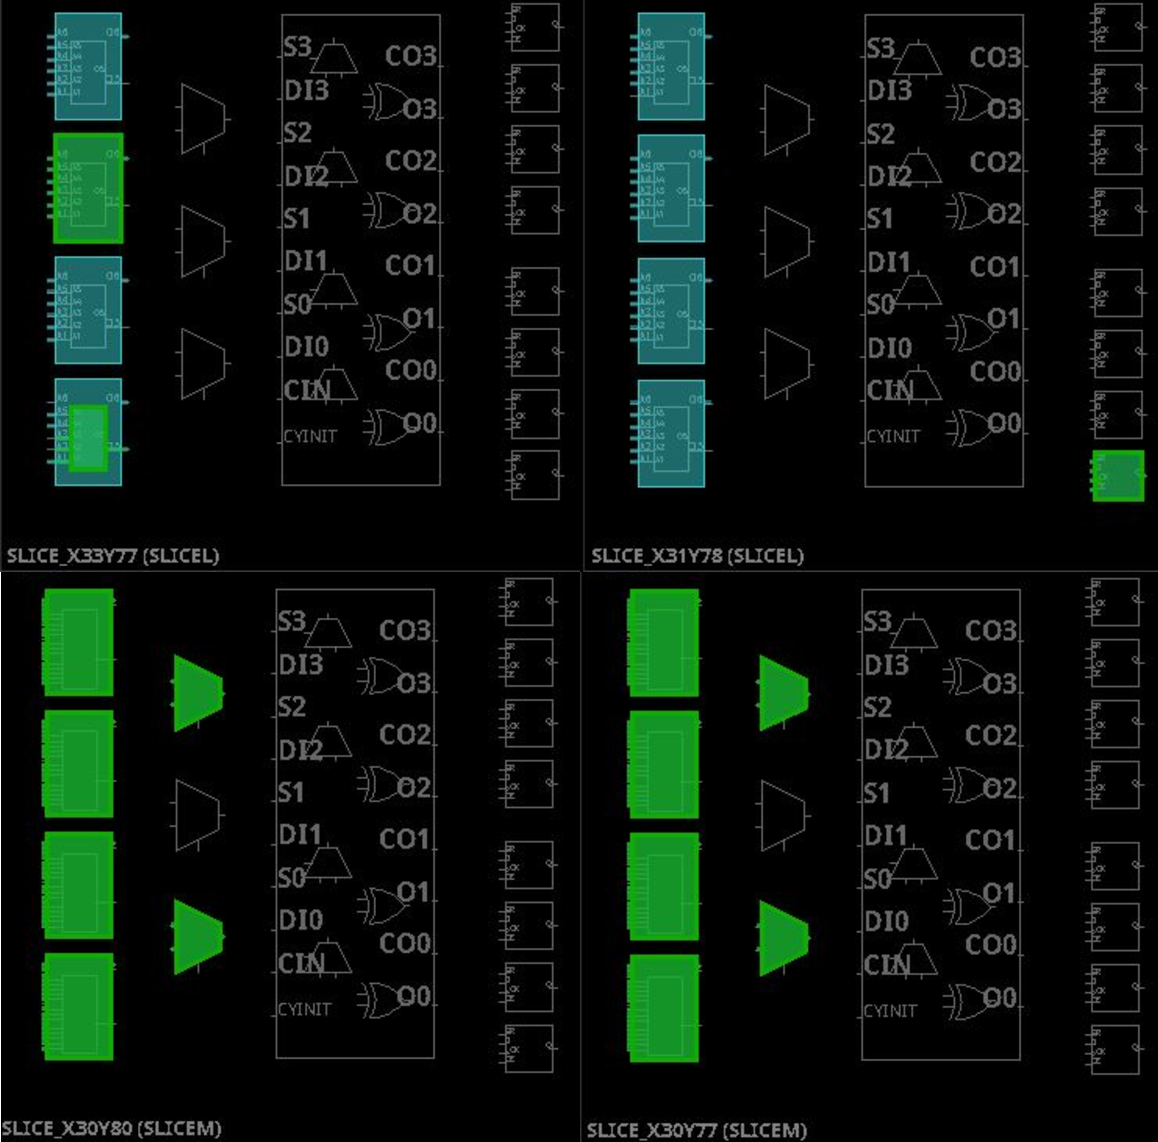
\includegraphics[width=0.6\linewidth]{images/SLICES.pdf}
            \caption{Slice composition of a single PE. Top two slices are SLICEL, bottom two are SLICEM; PE resources are highlighted in green neighbouring PE resources in teal.}
            \label{fig:SLICES}
        \end{figure}
    
        \subsubsection{Cycles per Instruction and Cycle Breakdown by FSM State}\label{sec:CPI}
            The comparison of cycles per instruction are shown in Table \ref{table:cpi_comparison}.
            \begin{table}[H]
                \centering
                \caption{Theoretical vs Measured CPI by Instruction}
                \label{table:cpi_comparison}
                \begin{tabularx}{\linewidth}{XXX}
                    \toprule
                    \textbf{Instruction} & \textbf{Theoretical CPI} & \textbf{Measured CPI} \\
                    \midrule
                    LOAD                    & 18 & 30 \\
                    STORE                   & 18 & 30 \\
                    R-Type (ADD/SRA/GETMSB)    & 17 & 29 \\
                    NEWS-Type              & 17 & 29 \\
                    \bottomrule
                \end{tabularx}
            \end{table}

            The theoretical cycle counts are derived from the number of states associated with each instruction in the FSM (Figure~\ref{fig:FSM}). It can be observed that the measured CPI is consistently 12 cycles higher than the theoretical values. This discrepancy arises from the overhead introduced by the AXI-Lite interface when transmitting instructions, which adds a fixed latency to each operation.

            Figure~\ref{fig:fsmPercentages}, illustrates the normalised cycle distribution across each FSM for both the Sobel and number classification workloads. In this case, arithmetic includes both R-Type and NEWS-Type instructions, I/O includes load and store operations, and IDLE refers to periods when the processor is not executing any instructions. Note that the MNIST cycle distribution is measured on the 16×16 configuration, while Sobel is measured on 32×32.
            
            \begin{figure}
                \centering
                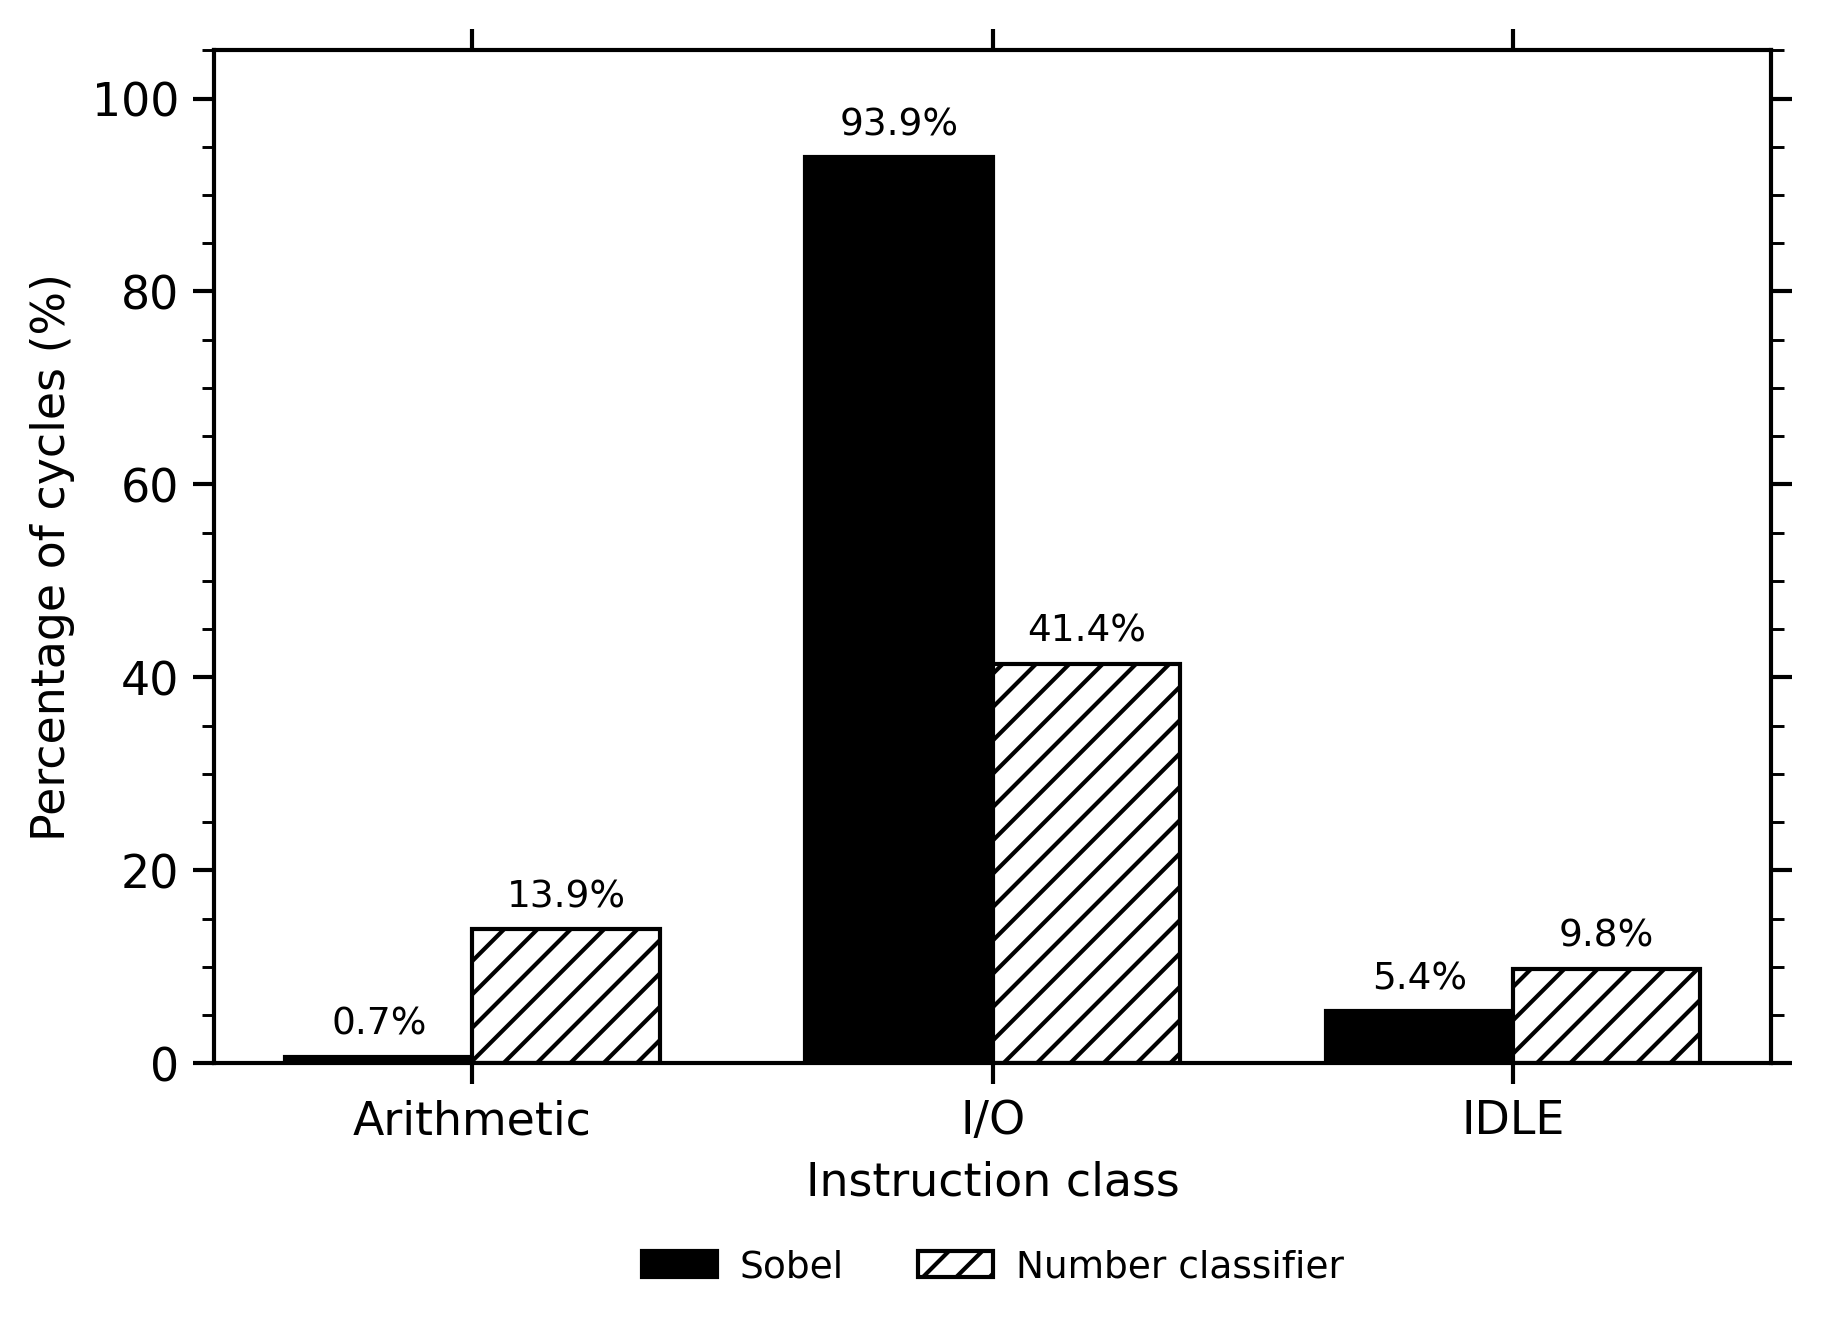
\includegraphics[width=0.7\linewidth]{images/FSMcycles.png}
                \caption{Cycle distribution by FSM state for the Sobel and number-classification workloads. The Sobel filter is executed on the 32×32 (1024-PE) configuration; the classifier is executed on the 16×16 (256-PE) configuration. Arithmetic combines R-type and NEWS-type instructions; I/O combines load and store; IDLE counts cycles in which no instruction is executing.}
                \label{fig:fsmPercentages}
            \end{figure}
            
        The cycles are expected to be dominated by I/O instruction types, since each pixel in a 32×32 image requires both a load and a store operation. (1024 loads and stores for the 32×32 Sobel image, and 256 for the 16×16 MNIST image). Hence, most instructions will be allocated to memory while only a few are arithmetic based ones. This memory bottleneck is a direct consequence of the single-word PISO/SIPO interface, and is revisited in Section~\ref{sec:bottleneck}.
        
        This effect is shown more clearly when comparing the Sobel workload against the simple image classifier. In the classifier algorithm, there are proportionally more arithmetic instructions for the same number of loads and stores, which is reflected in the shift from 0.7\% arithmetic cycles in Sobel to 13.9\% for the number classifier. Correspondingly, the memory share drops from 93.9\% to 41.4\%, indicating that the classifier is significantly more compute-bound than the Sobel edge detector. The IDLE share also grows slightly, from 5.4\% in Sobel to 9.8\% for the number classifier. This is due to the increased per-instruction handshaking overhead incurred by a longer instruction stream.

        \subsubsection{Throughput} \label{sec:throughput}
            The array's peak computational throughput is reported in bit-serial giga-operations per second (GOPS). Each of the 1024 PEs produces one bit-level operation per clock cycle during arithmetic execution so the peak bit-operation rate of the array is given by
            
            \begin{equation}
            \text{OPS}_{bit} = N_\text{PE} \times f_\text{clk},
            \end{equation}
            
            where $\text{OPS}_{bit}$ is the bit-level operation rate, $N_\text{PE}$ is the number of PEs (1024), and $f_\text{clk}$ is the maximum clock frequency (71 MHz). This yields a peak throughput of approximately 72.7 GOPS.
            
            However, this represents the theoretical maximum bit-level activity and does not account for instruction-level execution overhead. Each instruction requires multiple clock cycles to complete, meaning that new operations are only issued once per instruction cycle.
            
            The effective word-level throughput can therefore be expressed as
            
            \begin{equation}
            \text{OPS}_{eff} = \frac{N_\text{PE} \times f_\text{clk}}{\text{CPI}} = \frac{1024 \times 71 \times 10^6}{30} \approx 2.42~\text{GOPS}.
            \end{equation}
            
            where $\text{OPS}_{eff}$ represents the effective instruction-level operation rate excluding the AXI handshake, and CPI is the average cycles per instruction.

           The max operating frequency is bounded by a critical path originating at the state register in the control unit and traversing to the MSB of the SIPO output register. The total delay along this route is 13.70~ns leaving 58~ps of positive slack. The delay is dominated by routing ($\approx$82\%) rather than logic ($\approx$18\%), reflecting the spatial spread of the PE array across the fabric.

    
    % ============================================================
    \subsection{Array Size Sweeps} %make log scale
    \label{sec:scaling}
    This section goes through how the metrics of the array are affected by scaling the array size from a size of 2 x 2 (4 PEs) to 32 x 32 (1024 PEs).

    \begin{figure}[H]
        \centering
        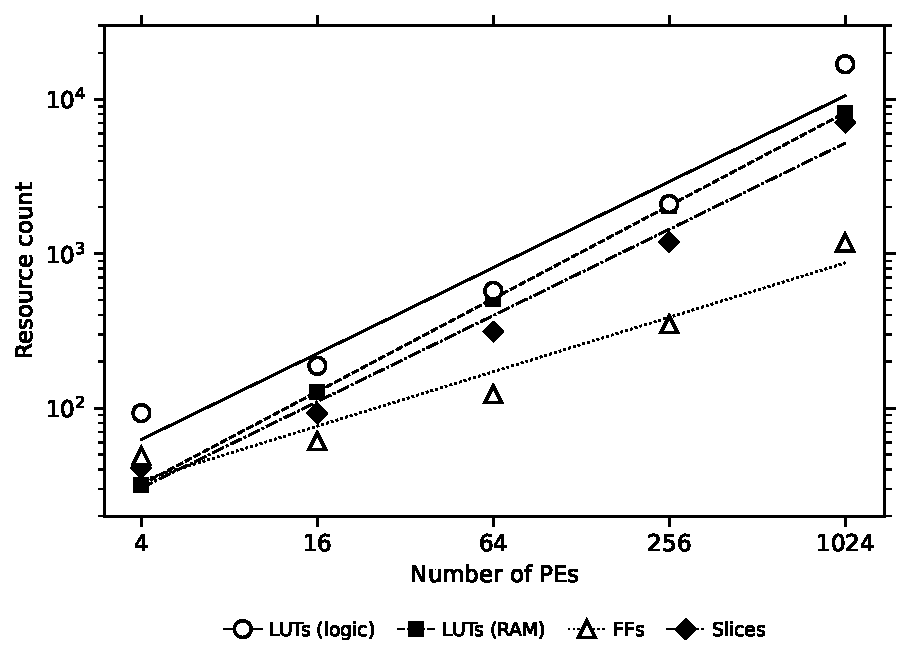
\includegraphics[width=0.6\linewidth]{images/ResourcevsPE.pdf}
        \caption{FPGA resource utilisation as a function of array size. Logic LUTs, LUTRAMs, flip-flops, and slices are reported for five PE configurations (4, 16, 64, 256, 1024). Lines are linear regressions in log–log space.}
        \label{fig:resource_scaling}
    \end{figure}
    
    Figure~\ref{fig:resource_scaling} shows the resource scaling across the five configurations. The trendline for LUTRAM count is linear line of unit slope, indicating linear scaling with PE count. This is the expected behaviour as the distributed register file in each PE does not interact across PEs and cannot be merged by the synthesiser. The slope for the flip-flop count is the lowest as each PE only contains 1 FF. On the other hand, Logic LUTs and slices scale faster than the other resources, particularly at larger array sizes. Between 256 and 1024 PEs, the LUT count grows by roughly 8× for a 4× increase in PE count. This growth is driven by the higher amount of LUTs per slice and the OR-reduction tree, whose fan-out forces the placer to insert buffers. At 1024 PEs the design consumes 31.7\% of the XC7Z020's logic LUTs and 47.1\% of its LUTRAM, making LUTRAM the binding resource.

    
    \begin{figure}[H]
        \centering
        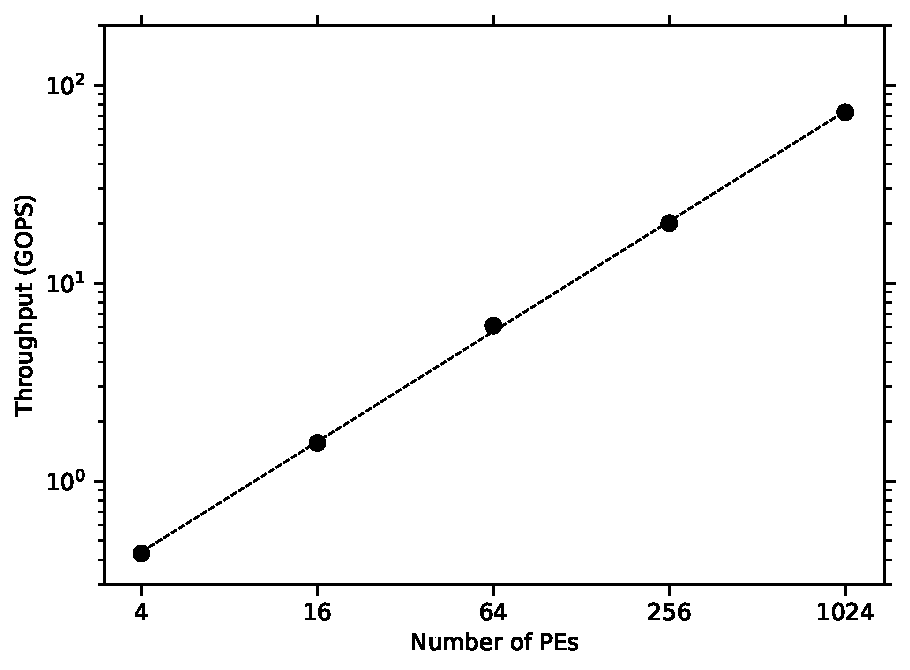
\includegraphics[width=0.6\linewidth]{images/GOPSvsPE.pdf}
        \caption{Theoretical peak bit-level throughput as a function of array size. The dashed line is a linear regression in log–log space}
        \label{fig:gops_scaling}
    \end{figure}
    
    Throughput, shown in Figure \ref{fig:gops_scaling}, is reported as the theoretical bit-level peak $\mathrm{GOPS} = F_\mathrm{max} \cdot N_\mathrm{PE}$, with each PE performing one bit-serial operation per cycle (note this is distinct from word-level throughput, which is lower based on the CPI.) The trendline has a gradient of 0.925, indicating a slightly sub-linear scaling. Throughput rises from 0.43 GOPS at 4 PEs to 72.92 GOPS at 1024 PEs; since each step increases the PE count by 4x, ideal scaling would yield a 4x speed-up per step, while the measured per-step speed-ups are 3.61x, 3.92x, 3.29x, and 3.63x. The shortfall is due to the degradation of the maximum clock frequency. $F_\mathrm{max}$ falls from 107.8~MHz at 4 PEs to 71.2~MHz at 1024 PEs, a 34\% reduction. 
    
    \begin{figure}[H]
        \centering
        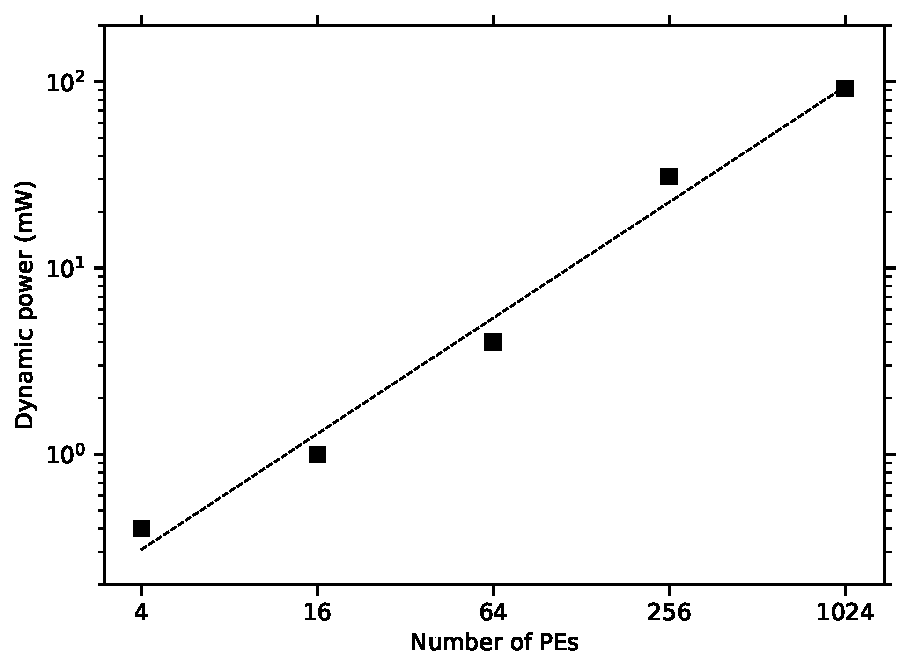
\includegraphics[width=0.6\linewidth]{images/PowervsPE.pdf}
        \caption{Dynamic power consumption as a function of array size. Power is reported for the array and control unit only, measured using a vectorless method. The dashed line is a linear regression in log–log space}
        \label{fig:power_scaling}
    \end{figure}
    
    Figure~\ref{fig:power_scaling} shows dynamic power of the processor (control and array) rising from 0.4 mW at 4 PEs to 92~mW at 1024 PEs. Similar to metrics described in the sections above, switching activity scales proportionally to PE count. Combining word-level throughput and power gives a peak energy efficiency of 0.0507 GOPS/mW at 16 PEs which degrades to 0.0264 GOPS/mW at 1024 PEs. This reduction in energy is due to the effects of sub-linear throughput scaling and the routing and fan-out overhead as mentioned in previous sections. Hence, for workloads prioritising energy efficiency over raw throughput, a configuration of 64-256 PEs offers a better operating point than the maximum array.

    \subsection{Resultant Images} \label{sec:imageResults}
    
    Figure \ref{fig:LenaEye} shows the processor implementing Sobel Edge detection. Overall, the algorithm requires 4.28 $\mu$s to complete at a frequency of 71 MHz. However, if I/O instructions are included, the total time for the program to complete is 870 $\mu$s

    \begin{figure}[H]
        \centering
        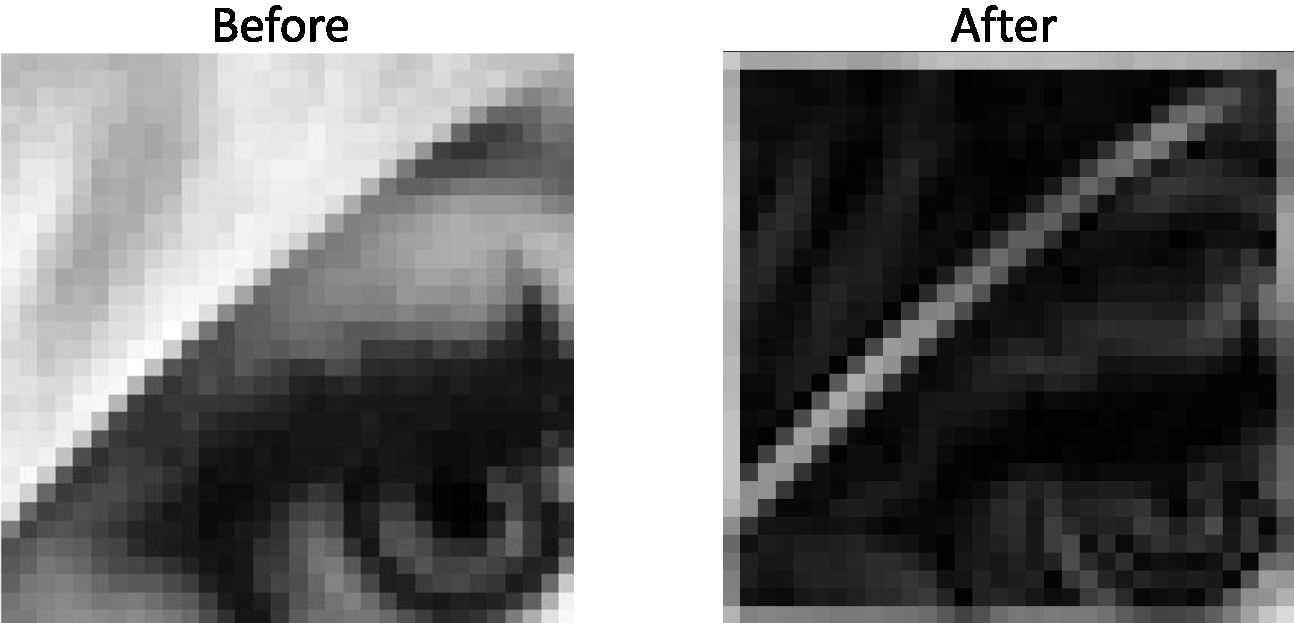
\includegraphics[width=0.75\linewidth]{images/LenaEye.pdf}
        \caption{Sobel edge detection on a 32x32 picture of an eye. Input shown on the left. Result shown on the right }
        \label{fig:LenaEye}
    \end{figure}

    Figure \ref{fig:MNIST_Eight} shows the processor running a simple CNN on the digit eight (shown in the left). The results (shown on the figure to the right) displays the calculated weights for each digit, selecting the highest one to be the predicted digit. The algorithm requires 109 $\mu$s to complete at a frequency of 71 MHz. However, if I/O instructions are included, the total time for the program to complete is 975 $\mu$s
    
    \begin{figure}[H]
        \centering
        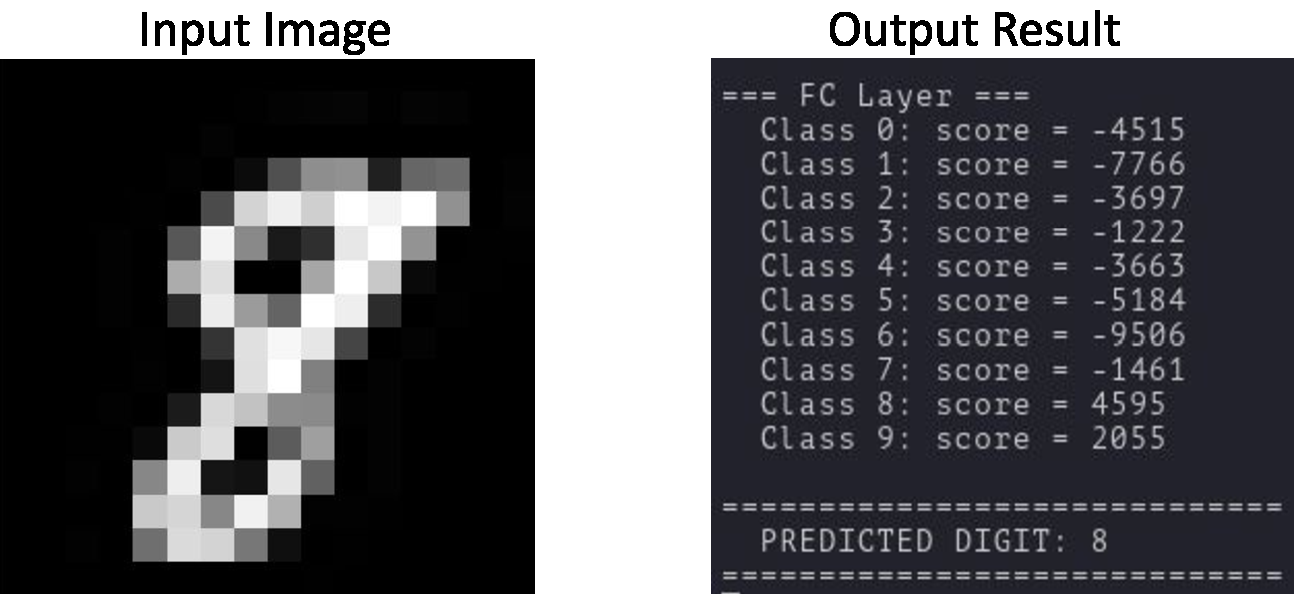
\includegraphics[width=0.75\linewidth]{images/MNIST_Eight.pdf}
        \caption{Number classification for the 16x16 digit eight. Input shown on the left. Result shown on the right}
        \label{fig:MNIST_Eight}
    \end{figure}

    \subsection{Comparison Against Prior Bit-Serial SIMD Designs}
    \label{sec:comparison}

    Direct comparison against the architectures surveyed in Chapter~\ref{sec:Literature Review} is bounded by differences in fabrication target, arithmetic precision, and reported metrics. The comparisons to be made in this section will be those that utilise a bit-serial SIMD design.

    The closest direct comparator is the bit-serial array of Walsh and Dudek~\cite{ref:walsh2012}, which targets a older Virtex-5 FPGA with bit-serial PEs with NEWS connectivity. The two designs achieve comparable per-PE footprints (3 - 4 slices versus 4), but Walsh's reaches a substantially higher operating frequency (150 MHz vs 71 MHz). Walsh's design does not include AXI-Lite host integration or the system wrapper used here, which adds per-instruction latency. The present work extends Walsh's design in two ways: shift-and-add convolution support in the ISA, enabling CNN workloads beyond Walsh's boolean and integer arithmetic, and integration into a complete ARM-host system.

    SPAR-2~\cite{ref:spar2} and IMAGine~\cite{ref:imagine} take a different approach, pairing bit-serial ALUs with distributed BRAMs in a processing-in-memory. This avoids the OR-tree bottleneck identified in Section~\ref{sec:bottleneck} and reaches frequencies up to 737 MHz, more than 10x the 71 MHz achieved here. However, it trades the pixel-to-PE locality that makes the present design efficient on Sobel and CNN convolutions. SCAMP-5~\cite{ref:scamp5} retains the strongest energy efficiency at 0.535 GOPS/mW as it uses mixed-signal ASIC fabrication, against the 0.0507 GOPS/mW peak measured here (Section~\ref{sec:scaling}).
    
    \subsection{Discussion}
    \label{sec:discussion}
    \subsubsection{Bottleneck Analysis} \label{sec:bottleneck}
    Overall, the results exposes three bottlenecks:

    It is evident that the dominant limiting factor for performance is the single word memory interface. Every word that goes into and out of the array has to be serialised through PISO/SIPO registers across the data width. This is why Sobel spends 93.9\% of its cycles in memory states while the number classifier, with its higher arithmetic intensity, drops to 41.4\% (Table \ref{fig:fsmPercentages}).
    
    The second bottleneck is the OR-reduction output tree, whose depth grows as $\log_2(N_\text{PE})$. The measured $F_\mathrm{max}$ reduction from 107.8 MHz to 71.2 MHz from 4 to 1024~PEs tracks this growth directly. Furthermore, the sharp rise in logic LUTs between 256 and 1024 PEs reflects the placer replicating drivers and inserting buffers on the high-fan-out nets feeding the tree.
    
    The third bottleneck is the Axi-Lite protocol latency, responsible for the uniform +12-cycle gap between theoretical and measured CPI (Table \ref{table:cpi_comparison}). As this cost occurs for every instruction, it grows as the array grows. The time spent in the IDLE state rising from 5.4\% to 9.8\% between Sobel and the number classifier demonstrates that a longer instruction stream pays this tax more often.
    
    \subsubsection{Implications for Design Improvements}
    The most effective change is to widen the memory interface, replacing the single PISO with a per-column bank so that a full row can be loaded in a number of cycles equal to the data width rather than scaling with both the number of columns and the data width. For the 32x32 array this reduces the per-image load/store cost by a factor of 32 and would bring Sobel's memory share down toward the 41.4\% figure seen in the number classifier case. Since LUTRAM rather than logic LUTs is the binding resource, and shift registers map efficiently to SRLs on the XC7Z020, this widening is affordable on the existing device.
    
    The second improvement is to pipeline the OR-reduction tree. Inserting a register stage every few levels would decouple $F_\mathrm{max}$ from array size at the cost of one added cycle per stage on the STORE path. This is negligible relative to the data width cycle serial transfer it feeds. This would remove the $F_\mathrm{max}$ cliff observed beyond 256 PEs and restore near-linear throughput scaling.
    
    The third improvement targets the instruction delivery path in the system level design. An instruction buffer placed between the ARM core and the processor would remove its lockstep. The buffer will be filled infrequently by the host and drained autonomously by the FSM, eliminating the per-instruction AXI-Lite handshake.
    
    \subsubsection{Threats to Validity}
    $F_\mathrm{max}$ was obtained under Vivado's default implementation strategy, so the 34\% degradation between 4 and 1024 PEs reflects tool effort rather than a silicon limit, and directed optimisation could likely recover part of it. Post-route power was measured using the default switching activity set by Vivado, so the reported GOPS/mW figures should be treated as indicative rather than measured values tied to a particular workload. Finally, kernels with intermediate intensity or unusual NEWS traffic patterns may show cycle distributions not captured in Figure~\ref{fig:fsmPercentages} where only Sobel and number classification workloads were employed. The cross-workload comparisons in Section \ref{sec:CPI} are normalised per workload to remain meaningful however, running both workloads on a single configuration would simplify direct comparison.


%%%%%%%%%%%%%%%%%% Project Manangement %%%%%%%%%%%%%%%%%%        
\section{Project Management} \label{sec:ProjectManagement}
    The project was structured around a Project Plan and Gantt chart (Appendix~\ref{sec:Gantt_Chart}) made before any work was started, defining the objectives and milestones to be completed. The Gantt chart was used as a dynamic tracker rather than something static: it was reviewed before supervisor meetings and when large changes to the project were required, providing a clear visual of completed work against planned work and helping both the author and his supervisor decide the scope and direction for each meeting.
    
    In the first semester, job interviews occurred at short notice, mitigated by front-loading tasks into earlier weeks to leave slack for later. Learning from prior projects, more work was allocated to the design stages to reduce bugs during implementation; the literature review and design overran the allocated two weeks, and a compromise was made to carry these out in parallel with prototyping simpler RTL modules. A laptop failure later caused loss of data and applications, requiring working hours to be extended into the Easter break.
    
    Risks were tracked in the Risk Register (Appendix~\ref{sec:RiskReg}), which compared each risk against its likelihood, impact, and mitigation strategy, with entries identified by analysing mistakes from previous projects. Key entries included tool-chain and data loss (mitigated through version control) and delays from external activities (mitigated by parallel task execution). The Health \& Safety Risk Assessment (Appendix~\ref{sec:H&S}) addressed risks to the author from prolonged desk-based work and the electrical safety considerations of FPGA bench use.
    
    Self-directed learning is documented in the CPD Log (Appendix~\ref{sec:CPD}) and played an important part in the project. Competence in SystemVerilog, bit-serial arithmetic, and Vivado synthesis was developed independently through textbooks, IEEE papers, and targeted online courses. Each significant new skill was logged with its source, application, and a short reflection on how it influenced subsequent design choices, providing a traceable link between learning activity and project outcomes.
    
    Initiative is most clearly evidenced by the response to finishing the Sobel edge-detection demonstration ahead of schedule. Rather than announcing the project was completed, the possibility of extending the instruction set to support image-classification inference on the array, alongside future novel ideas, was proposed to the supervisor with a view to potential future publication. This required re-scoping the remaining Gantt entries, updating the Risk Register with new technical risks, and committing to additional independent study.
      

%%%%%%%%%%%%%%%%%% CONCLUSIONS %%%%%%%%%%%%%%%%%%
\section{Conclusions and Future Work}\label{sec:conclusion}
    This section presents the conclusions drawn from researching and designing this array processor and the improvements that can be taken to address its limitations.
    
    \subsection{Conclusion}
        Of the five objectives defined in Section \ref{sec:aims}, four were met in full and one was met partially. Against Objective \ref{item:obj1}, a parametrised bit-serial PE was designed and verified, occupying 3 to 4 slices per PE with a constant 8 LUTRAMs and 1 carry flip-flop, a per-PE footprint comparable to the four-slice cost reported by Walsh and Dudek \cite{ref:walsh2012}. Against Objective \ref{item:obj2}, each PE was replicated into a NEWS-connected array, demonstrating that scaling from 4 to 1024 PEs on the XC7Z020 was possible, with the maximum 32×32 configuration consuming 31.7\% of the available logic LUTs and 47.1\% of LUTRAM. Against Objective \ref{item:obj3}, a hardware control unit and 20-bit ISA covers all four instruction classes with reliable handshaking communication between the ARM core and the processor. Against Objective \ref{item:obj4}, the array was integrated with an ARM Cortex-A9 over AXI-Lite and a true-dual-port BRAM, and against Objective \ref{item:obj5}, both Sobel edge detection at 32×32 and MNIST classification at 16×16 produced correct output. It is worth mentioning the caveat associated with the MNIST workload here: the convolution, ReLU, and max-pooling stages execute on the array, but the final fully connected layer runs on the ARM host because the ISA trades multiply-accumulate support for area efficiency and simplicity. The classifier is therefore a hybrid between the host and acceleration rather than a fully on-array CNN.
    
        Against the three evaluation criteria, the picture is mixed. Area efficiency was the most successful criteria, with each PE taking up comparable area with other bit-serial array FPGA implementations. Furthermore, the full 1024-PE array fits within the target device alongside with its supporting infrastructure. Performance scales with PE count, from 0.43 GOPS at 4 PEs to 72.92 GOPS at 1024 PEs at 71.2 MHz, but sub-linearly with a 34\% $F_\mathrm{max}$ degradation across the sweep; the headline figure is also a theoretical peak, with effective instruction-level throughput at 2.42 GOPS and Sobel spending 93.9\% of cycles in memory states. Power efficiency peaks at 0.0507 GOPS/mW (16 PEs) and settles to 0.0264 GOPS/mW at 1024 PEs.

    \subsection{Future Work}\label{sec:futwork}
        From an architectural standpoint, the current design employs a two-dimensional mesh interconnect which, while area-efficient, incurs significant latency penalties for non-local data movement. Examples of this include the stride two calculations after the first max pooling layer. Extending the interconnect to support a richer topology, such as a hypercube or a hierarchical mesh similar to that employed in the CM-2, would reduce worst-case hop counts and improve the performance of operations that require broader spatial context.
        
        The bit-serial datapath, while central to the area efficiency of the architecture, imposes a fundamental limit on per-operation latency. The next steps for future work would be to investigate a configurable bit-width mode, in which groups of PEs could be dynamically reconfigured to operate in a bit-parallel fashion for latency-critical operations and revert to bit-serial operation for bulk workloads. A mode for variable precision further allows for a higher throughput 
        
        Finally, integration with on-chip or near-sensor memory, in the spirit of the SCAMP-5 pixel processor array, represents an attractive long-term direction. By co-locating sensing, memory, and computation, the memory bandwidth bottleneck that constrains many edge-intelligent systems may be substantially reduced. Migrating the design from its current FPGA prototype to an ASIC implementation would also permit a more accurate assessment of its power and area efficiency and would enable direct comparison with the historical and modern arrays reviewed in this report.
    

%%%%%%%%%%%%%%%%%% REFERENCES %%%%%%%%%%%%%%%%%%
%\clearpage % uncomment to start on a new page if wanted
\printbibliography[title={References},heading=bibintoc] % a single list of references for the whole thesis



%%%%%%%%%%%%%%%%%% APPENDICES %%%%%%%%%%%%%%%%%%
\begin{uomappendix} 

    \section{Preliminary Project Proposal} \label{sec:ProjectProposal}
    \subsection{Background}
    
        Image processing is the core workload of various edge systems. 2D convolution is the fundamental operation found in low-level vision and convolutional neural network (CNN) tasks. This is where a weighted sum of a pixel and its neighbours are repeated across the entire image. A single 3×3 convolution on a modest 256×256 image already requires over half a million multiply-accumulate (MAC) operations, and modern CNNs scale this by orders of magnitude through multiple stacked convolutional layers and feature channels. Executing such workloads on conventional sequential processors is very inefficient. Pipelining, superscalar issue, and out-of-order execution all target instruction-level parallelism, but they do not exploit the property that the same operation is ap- plied independently to many data elements.
            
    \subsection{Motivation}
    
    Single-Instruction-Multiple-Data (SIMD) array processors exploit this property directly. A grid of processing elements (PEs) executes one shared instruction across many pixels in parallel, elimi- nating the per-instruction fetch and decode cost. When the array is connected through nearest- neighbour links, the spatial structure of convolution maps onto the hardware without the need for global memory access.
    
    \subsection{Aim}
    
    The aim of this project is to design, implement, and evaluate an FPGA-based bit-serial SIMD array processor capable of executing image-processing workloads.
    
    \subsection{Objectives}
    
    \begin{enumerate}
        
        \item \textbf{Bit-serial processing element:}\label{item:obj1} Design a simple processing element comprising a bit-serial ALU supporting arithmetic and boolean logic alongside a bit-serial register file. Success is defined as a functionally correct Processing Element (PE) that passes testcases across all supported ALU operations and performs proper reads and writes to the register file, while achieving a per-PE slice and Look-Up-Table (LUT) footprint competitive with prior bit-serial FPGA designs.
        
        \item \textbf{Scalable NEWS-connected array:}\label{item:obj2} Replicate the PE into a two-dimensional grid with North, East, West, South (NEWS) connectivity, with a configurable boundary padding scheme and PE activity gating for inactive elements. Success is defined as fitting a large array configuration, sized against current bit-serial processors, within the available resources, delivering throughput in GOPS that scales with PE count while keeping dynamic power consumption (in mW) low enough to yield a competitive GOPS/mW figure.
        
        \item \textbf{Hardware control unit and instruction set architecture:}\label{item:obj3} Develop an FSM-based controller with a minimal instruction set sufficient to run complex workloads, sequence bit-serial PE execution, and provide a ready/valid handshake to the host. Success is defined as full ISA coverage through workload execution, with the controller correctly driving all datapath control signals.
        
        \item \textbf{ARM-host system integration:}\label{item:obj4} Connect the array processor to the ARM Cortex-A9 on the PYNQ-Z2 using AXI-Lite for instruction delivery and a true-dual-port BRAM for data exchange. Success is defined as a working host-accelerator system in which C programs running on the ARM core can issue instructions and read back results, with the integration logic fitting within the target device alongside the full array.
        
        \item \textbf{Application demonstration and evaluation:}\label{item:obj5} Implement two image processing workloads on the completed system: a 3x3 Sobel edge-detection filter and a shallow convolutional neural network for MNIST digit classification. Success is defined as both workloads producing the expected results: visible edges in the Sobel output and predicted digits matching the input labels.
        
        \end{enumerate}


    \section{Project Plan and Gantt Chart} \label{sec:Gantt_Chart}
        The section that follows lays out the project plan and the Gantt charts for semesters one and two (shown in figure \ref{fig:Sem1Gantt} , \ref{fig:Sem2Gantt})



        \begin{figure}[H]
            \centering
            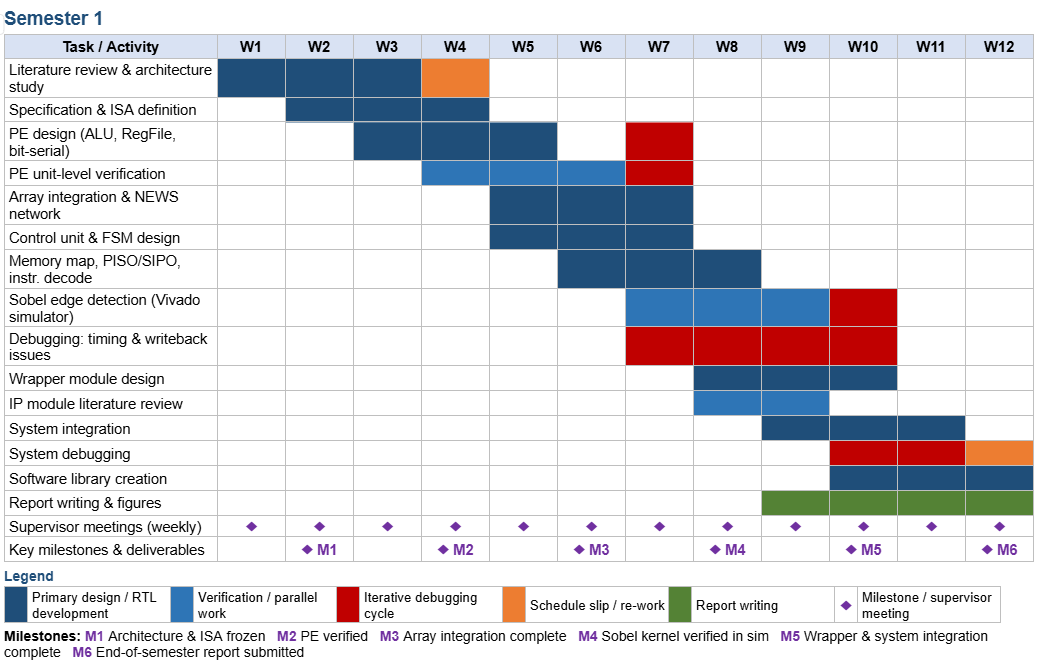
\includegraphics[width=\linewidth]{images/Sem1Gantt.png}
            \caption{Gantt chart for the bit-serial array processor during semester 1}
            \label{fig:Sem1Gantt}
        \end{figure}
        
        \begin{figure}[H]
            \centering
            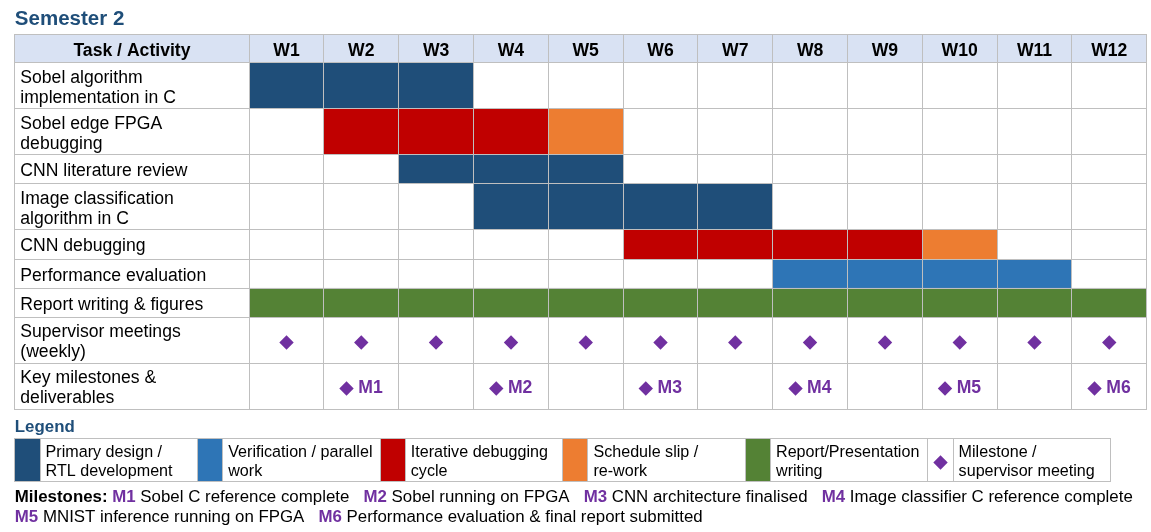
\includegraphics[width=\linewidth]{images/Sem2Gantt.png}
            \caption{Gantt chart for the bit-serial array processor during semester 2}
            \label{fig:Sem2Gantt}
        \end{figure}
    
    \section{Health and Safety Risk Assessment}\label{sec:H&S}
        Figure \ref{fig:RiskAssessment} analyses the different hazardous activities that will appear when taking on this project, mitigation strategies and the risk level associated with each risk.
    
        \begin{figure}[H]
            \centering
            
\includegraphics[width=\linewidth]{images/RiskAssessment.png}
            \caption{Risk Assessment Form}
            \label{fig:RiskAssessment}
        \end{figure}
        
    \section{Risk Register}\label{sec:RiskReg}
        Figure \ref{fig:RiskReg} shows the associated risks that will affect the progression of the project.
        
        \begin{figure}[H]
            \centering
            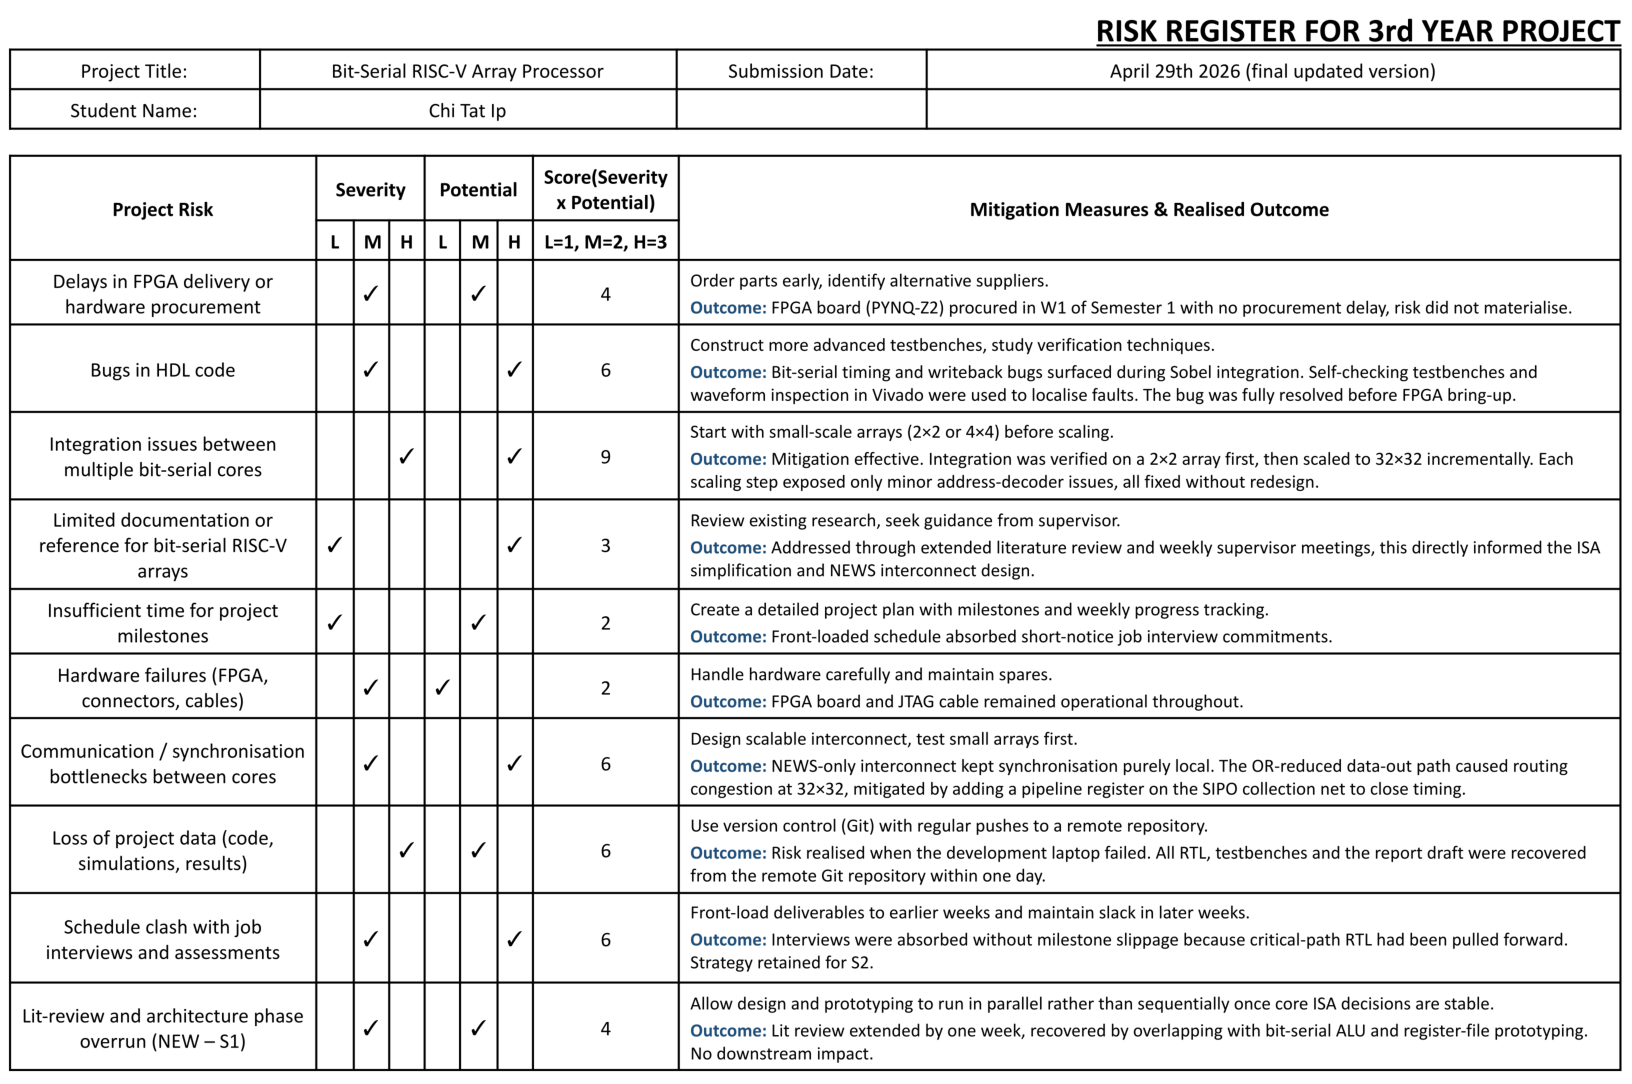
\includegraphics[width=\linewidth]{images/RiskRegister.pdf}
            \caption{Risk Register}
            \label{fig:RiskReg}
        \end{figure}

    \section{Continuing Professional Development Log}\label{sec:CPD}
        
        The Continuing Professional Development (CPD) log shown in Figure~\ref{fig:CPD} summarises the technical learning activities that have been taken already and those that are planned for the future.
        
        \begin{figure}[H]
            \centering
            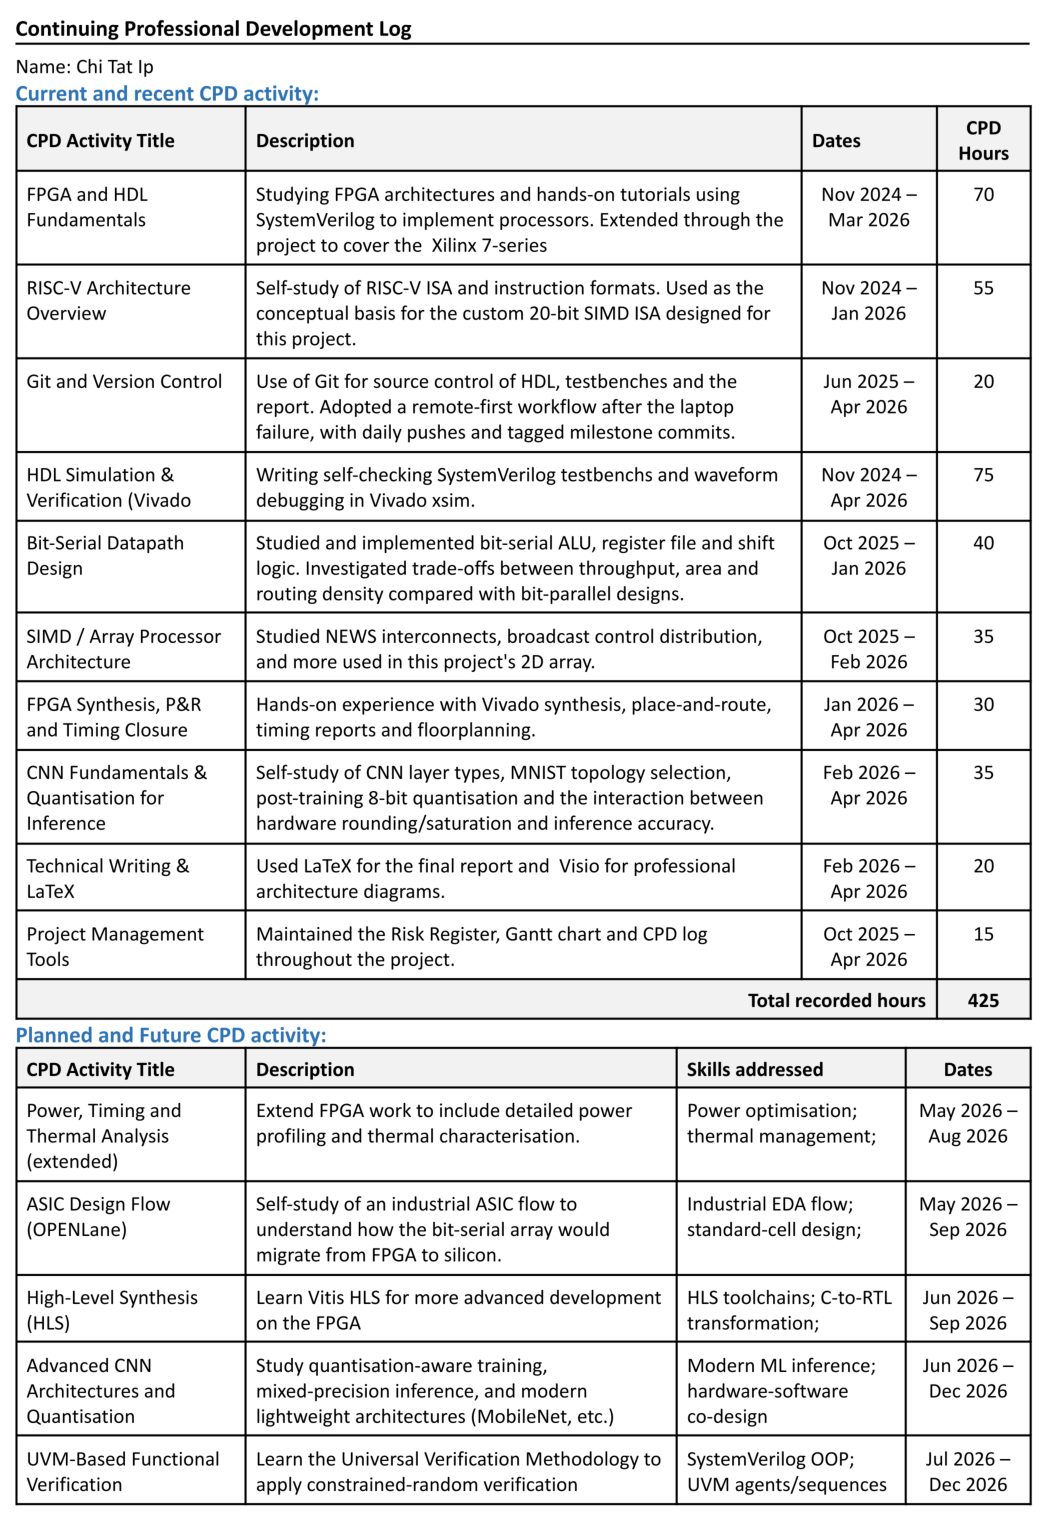
\includegraphics[width=0.85\linewidth]{images/CPD.pdf}
            \caption{Continuing Professional Development (CPD) log}
            \label{fig:CPD}
        \end{figure}

    
    \section{Github Repository}\label{sec:GitHub}
    The repository containing entire project is separated into two repositories. The repository name "Individual-Project" contains the SystemVerilog design of my array processor,  verification directories, and custom IPs. The repository labeled "Individial\_Project\_System" contains the hardware description for the system level design as well as the C program used to communicate with the array processor through the ARM processor to run image classification.

    \textbf{Array Processor:} \url{https://github.com/adho-bot/Individual_Project}\\ 
    \textbf{System Design and Software:} \url{https://github.com/adho-bot/Individual_Project_System}

    \section{Derivation of the General Movement-Based Convolution Formula}
    \label{app:conv_derivation}
    
    For a continuous image $f(x,y)$ and a kernel $h(x,y)$, the 
    two-dimensional convolution is defined as
    
    \begin{equation}
    (f * h)(x,y) =
    \int_{-\infty}^{\infty}
    \int_{-\infty}^{\infty}
    f(u,v)\,h(x-u,y-v)\,du\,dv
    \label{eq:continuous_convolution}
    \end{equation}
    
    For a digital image $I(x,y)$ and discrete kernel $K[m,n]$ of size 
    M x N, the convolution becomes
    
    \begin{equation}
    C(x,y)=
    \sum_{m=-p}^{p}
    \sum_{n=-q}^{q}
    k_{m,n}\,I(x-m,y-n),
    \quad
    p=\frac{M-1}{2},\;
    q=\frac{N-1}{2}
    \label{eq:discrete_convolution}
    \end{equation}
    
    For a 3x3 kernel where $M=N=3$ and $p=q=1$, 
    Equation~\eqref{eq:discrete_convolution} becomes
    
    \begin{equation}
    C(x,y)=
    \sum_{i=-1}^{1}
    \sum_{j=-1}^{1}
    k_{i,j}\,I(x+j,y+i)
    \label{eq:conv_3x3}
    \end{equation}
    
    Expanding Equation~\eqref{eq:conv_3x3} yields
    
    \begin{equation}
    \begin{aligned}
    C(x,y) &= k_{-1,-1}I(x-1,y-1)
    + k_{-1,0}I(x,y-1)
    + k_{-1,1}I(x+1,y-1) \\
    &\quad + k_{0,-1}I(x-1,y)
    + k_{0,0}I(x,y)
    + k_{0,1}I(x+1,y) \\
    &\quad + k_{1,-1}I(x-1,y+1)
    + k_{1,0}I(x,y+1)
    + k_{1,1}I(x+1,y+1)
    \end{aligned}
    \label{eq:conv_expanded}
    \end{equation}
    
    
    \section{Array Processor Implementation of the Sobel Kernels}
    \label{app:sobel_derivation}
    
    Sobel edge detection uses two kernels that estimate the horizontal 
    and vertical image gradients
    
    \begin{equation}
    G_x =
    \begin{bmatrix}
    -1 & 0 & 1\\
    -2 & 0 & 2\\
    -1 & 0 & 1
    \end{bmatrix}
    \qquad
    G_y =
    \begin{bmatrix}
    -1 & -2 & -1\\
    0 & 0 & 0\\
    1 & 2 & 1
    \end{bmatrix}
    \label{eq:sobel_kernels}
    \end{equation}
    
    Applying Equation~\eqref{eq:conv_3x3} to the horizontal kernel $G_x$ 
    and ignoring zero terms gives
    
    \begin{equation}
    \begin{aligned}
    G_x(x,y) &= (-1)I(x-1,y-1) + 1I(x+1,y-1) \\
    &\quad + (-2)I(x-1,y) + 2I(x+1,y) \\
    &\quad + (-1)I(x-1,y+1) + 1I(x+1,y+1)
    \end{aligned}
    \label{eq:sobel_expanded}
    \end{equation}
    
    This expression can be rewritten as the difference between the east 
    and west column contributions
    
    \begin{equation}
    G_x(x,y)=I_{\text{east}}-I_{\text{west}}
    \label{eq:sobel_column_difference}
    \end{equation}
    
    where
    
    \begin{align}
    I_{\text{west}} &= I(x-1,y-1)+2I(x-1,y)+I(x-1,y+1)
    \label{eq:sobel_west}\\
    I_{\text{east}} &= I(x+1,y-1)+2I(x+1,y)+I(x+1,y+1)
    \label{eq:sobel_east}
    \end{align}
    
    To avoid multiplication, the weighting factor of two can be produced 
    using repeated summation of shifted images. First, a partial vertical 
    sum is constructed
    
    \begin{equation}
    B(x,y)=I(x,y)+I(x,y-1)
    \label{eq:partial_sum}
    \end{equation}
    
    Shifting this value south and adding again produces
    
    \begin{equation}
    C(x,y)=B(x,y)+B(x,y+1)
    \label{eq:column_sum}
    \end{equation}
    
    Expanding Equation~\eqref{eq:column_sum} gives
    
    \begin{equation}
    C(x,y)=I(x,y-1)+2I(x,y)+I(x,y+1)
    \label{eq:sobel_column_weight}
    \end{equation}
    
    which reproduces the vertical Sobel weighting without requiring 
    multiplication.
    
    The horizontal gradient can therefore be computed as
    
    \begin{equation}
    G_x(x,y)=C(x+1,y)-C(x-1,y)
    \label{eq:sobel_gx}
    \end{equation}
    
    The same procedure applied to $G_y$ yields the symmetric form, with 
    east/west sums replacing north/south and the final difference taken 
    between north and south neighbours.

    \section{Memory and Register Allocation for MNIST CNN Inference} \label{sec:memregalloc}


    \begin{table}[H]
        \centering
        \caption{BRAM word-address memory map.}
        \label{tab:bram_map}
        \begin{tabular}{lll}
        \hline
        \textbf{Region} & \textbf{Word Addresses} & \textbf{Contents} \\
        \hline
        Input image     & 0 -- 255      & Raw 16x16 pixel values \\
        Pooled channel 0 & 256 -- 304   & 7x7 max-pool output, filter 0 \\
        Pooled channel 1 & 320 -- 368   & 7x7 max-pool output, filter 1 \\
        \hline
        \end{tabular}
    \end{table}
        

    
    \begin{table}[H]
        \centering
        \caption{PE register allocation during CNN inference.}
        \label{tab:reg_alloc}
        \begin{tabular}{ll}
        \hline
        \textbf{Register} & \textbf{Purpose} \\
        \hline
        \texttt{r0} & Hardwired zero (identity for add-based moves) \\
        \texttt{r1} & Input image pixel / pooling operand \\
        \texttt{r2} & Convolution accumulator \\
        \texttt{r3} & Neighbourhood operand (shifted neighbour value) \\
        \texttt{r4} & Shift temporary / comparison result \\
        \texttt{r5} & Convolution filter 1 post-ReLU output \\
        \texttt{r6} & Convolution filter 0 post-ReLU output \\
        \texttt{r7} & All-ones mask (\texttt{0xFFFF}) \\
        \hline
        \end{tabular}
    \end{table}

    
\end{uomappendix}


%%%%%%%%%%%%%%%%%% END MATTER %%%%%%%%%%%%%%%%%%
\end{document}